\documentclass[a4paper,10pt]{report}

% Package import
\usepackage[a4paper,inner=3.5cm,outer=2.5cm]{geometry}
\usepackage[ngerman]{babel}
\usepackage[T1]{fontenc}
\usepackage[utf8]{inputenc}
\usepackage{epstopdf}

\usepackage{
} %Type1-Schriftart für nicht-englische Texte

\usepackage{amsmath}
\usepackage{amsthm}
\usepackage{amssymb}
\usepackage{graphicx}
\usepackage{mathtools}
\usepackage{tabularx}
\usepackage{framed}
\usepackage{float}


\newtheorem{mydef}{Definition}
\newtheorem{myexample}{Beispiel}
\newtheorem{myproof}{Beweis}
\newtheorem{axiom}{Axiom}

% Mathbox
\newenvironment{mathbox}
{\par\smallskip\centering\begin{lrbox}{0}%
\begin{minipage}[c]{\textwidth}}
{\end{minipage}\end{lrbox}%
\framebox[\textwidth]{\usebox{0}}%
\par\medskip
\ignorespacesafterend}

%  Code
\usepackage{listings}
\usepackage{color}

\definecolor{dkgreen}{rgb}{0,0.6,0}
\definecolor{gray}{rgb}{0.5,0.5,0.5}
\definecolor{mauve}{rgb}{0.58,0,0.82}

\usepackage{pbox}
\newcommand{\longcell}[2][c]{%
  \begin{tabular}[#1]{@{}c@{}}#2\end{tabular}}

\lstset{frame=tb,
  language=Java,
  aboveskip=3mm,
  belowskip=3mm,
  showstringspaces=false,
  columns=flexible,
  basicstyle={\small\ttfamily},
  numbers=none,
  numberstyle=\tiny\color{gray},
  keywordstyle=\color{blue},
  commentstyle=\color{dkgreen},
  stringstyle=\color{mauve},
  breaklines=true,
  breakatwhitespace=true
  tabsize=3
}
\lstset{language=Java}

% sets of numbers
\newcommand{\N}{{\mathbb N}}
\newcommand{\Z}{{\mathbb Z}}
\newcommand{\Q}{{\mathbb Q}}
\newcommand{\R}{{\mathbb R}}
\newcommand{\C}{{\mathbb C}}

% imaginary unit
\newcommand{\iu}{{i\mkern1mu}}


%% Zeilenabstand %%%%%%%%%%%%%%%%%%%%%%%%%%%%%%%%%%%%%%%%%%%%
%\usepackage{setspace}
%\singlespacing        %% 1-zeilig (Standard)
%\onehalfspacing       %% 1,5-zeilig
%\doublespacing        %% 2-zeilig


\begin{document}

\pagestyle{empty} %%Keine Kopf-/Fusszeilen auf den ersten Seiten.

%% Die einfache Version:
\title{Algorithmen und Datenstruktur}
\author{Martin Schmidli}
%\date{} %%Wenn kommentiert, wird das aktuelle Datum verwendet.
\maketitle


%% Inhaltsverzeichnis %%%%%%%%%%%%%%%%%%%%%%%%%%%%%%%%%%%%%%%
\tableofcontents %Inhaltsverzeichnis
\cleardoublepage %Das erste Kapitel soll auf einer ungeraden Seite beginnen.

\pagestyle{plain} %%Ab hier die Kopf-/Fusszeilen: headings / fancy / ...

%% Kapitel / Hauptteil des Dokumentes %%%%%%%%%%%%%%%%%%%%%%%

%-------------- Grundlagen --------------

\chapter{Algorithm}
Je nach Algorithmus dauert es länger eine Aufgabe zu lösen.
\section{Sort Algorithmen}
Ziel ist es eine Anzahl von $n$ Ganzzahlenwerten ihrem Wert nach zu Ordnen (0,1,2...).
\subsection{Bubblesort}
Diese Tatsache wird im Bubblesort Algorithmus ausgenutzt.\\
Um eine Liste mit n Zahlen zu sortieren, muss im Worst Case Szenario i = n-1 mal durch die Liste durchiteriert werden. In jedem Durchgang werden die Positionen der Zahlen überprüft. Ist die das erste Element grösser als das zweite Element wird deren Position getauscht. Ist die erste Zahle kleiner behält sie ihren Platz.\\
\\Der Algorithmus wird  Bubblesort genannt, weil die höchstwertigste Zahl sehr rasch an das Ende des Arrays  verschoben wird. Die Zahl schwebt nach oben resp. an das Ende des Arrays wie in einer Blase/''Bubble''. Nun müssen wir nicht jedes m mal durchiterieren, denn wir wissen, dass die Zahlen am Ende des Arrays bereits die richtige Position haben. 
\\
\\Bsp. Wir iterieren 2 mal durch das Array. Die 2 Letzten Zahlen im Array haben also die korrekte Position.\\
Aus diesem Grund überprüfen wir pro Durchgang immer eine Zahl weniger, i--.\\
\\
Java Implementation:
\begin{lstlisting}
/**
 * Non optimized bubble sort for an int array 
* @param a, array  of n integers which we would like to sort
*/
public static void bubbleSort(int[] a) {
	cnt=0;
	int m = a.length-1;
	for(int i=m; i>0; i--){ 
		for (int k=0; k < i; k++){
			if(a[k]>a[k+1]) swap(a,k,k+1);
		}
		// now a[i] is on its final position!
	}
}
\end{lstlisting}
Eine mögliche Verbesserung wäre es, ein ''isSorted'' Flag einzubauen. Wir überprüfen pro Durchgang i, ob wir geswapt haben. Wurden keine Zahlen vertauscht, ist das Array korrekt sortiert und wir können die Schleife abbrechen.
\newpage
\noindent
\subsection{Quicksort}
Der Quicksort Algoritmus ist meist sehr viel schneller als der Bubble Sort Algoithmus. Nur wenn die Liste bereits sortiert und dieser Spezialfall nicht abgefagen wird, sind Sie gleich schnell.
Das Grundproblem/ Aufgabe wird beim Quicksort in kleine Probleme zerlegt, wir sprechen von Partitionieren. In der Programmierung sprechen wir von Rekursion.\\
\\
Wir suchen uns ein zufälliges Element aus dem Array aus. Dieses Element wird Pivot genannt.\\
Wir tauschen das letzte Element des Arrays mit dem Pivot. Damit fangen wir den Spezialfall einer bereits sortierten Liste ab.\\
\\
Stellen wir uns zwei Zeiger ''Left'' und ''Right'' auf das Array vor. Left startet beim 1. Elements des Arrays, A[0]. Right startet beim Ende des Arrays [Anzahl Elemente-1]. Left fährt von Links nach Rechts. Der Index von Left wächst bis er auf ein Element zeigt, welches grösser ist als der Pivot. Right fährt von Rechts nach Links. Der Index von Right  wird kleiner, bis es auf ein Element kleiner als der Pivot zeigt. Die beiden Elemente bei A[Left] und A[Right] werden ausgetauscht.\\
\\
Dieser Ablauf wird fortgesetzt, bis die Zeiger aufeinander zeigen, Left == Right.\\
Alle kleineren Zahlen als der Pivot sind nun also auf der Linken Seite, alle grösseren auf der Rechten Seite des momentanen Indexes. Nun können wir den Pivot mit dem Element an dieser Stelle vertauschen.\\
\\
Wir haben die korrekte Position des momentanen Pivot gefunden.
Es ergebn sich nun zwei neue Bereiche. Links vom Pivot und Rechts vom Pivot.\\
Wir beginnen den Prozess von vorne.\\
Wir rufen die Funktion zweimal mit den neuen Bereichen (Begin,Left-1) und (Left+1, End) auf.\\
Der Prozess begint von vorne.\\
\\
Java Implementation:
\begin{lstlisting}
public static void quickSort(int[] a, int start, int end)
{
	int left = start;
	int right = end;
			
	// check if we have to do something
	if(end-start > 0)
	{		
		// move random to last index
		Random rand = new Random();
		int random = rand.nextInt((end-start)+1)+start;			
		swap(a,random,end);
		int pivot = a[end];			
		
		// we do move until the pointer are at the same position
		while(left < right)
		{
			// move left pointer until we found a bigger number as pivot
			while(left < right && a[left] <= pivot)
			{
				left++;
			}
			
			// move right pointer until we found a smaller number as pivot
			while(left < right && a[right] >= pivot)
			{
				right--;
			}
			
			// exit if pointer are at the same position
			if(left == right) break;
			
			// we found two numbers, lets swap them
			swap(a,left, right);
		}			
		//Move the pivot to his correct position
		swap(a, end,left);
		
		// Now we do have two new fields/ arrays. Lets call quickSort recursively
		quickSort(a, start, left-1);
		quickSort(a,left+1, end);
	}
}
\end{lstlisting}
\newpage
\section{Trees}
Preorder Traversal
\begin{figure}[H]
	\begin{center}
  		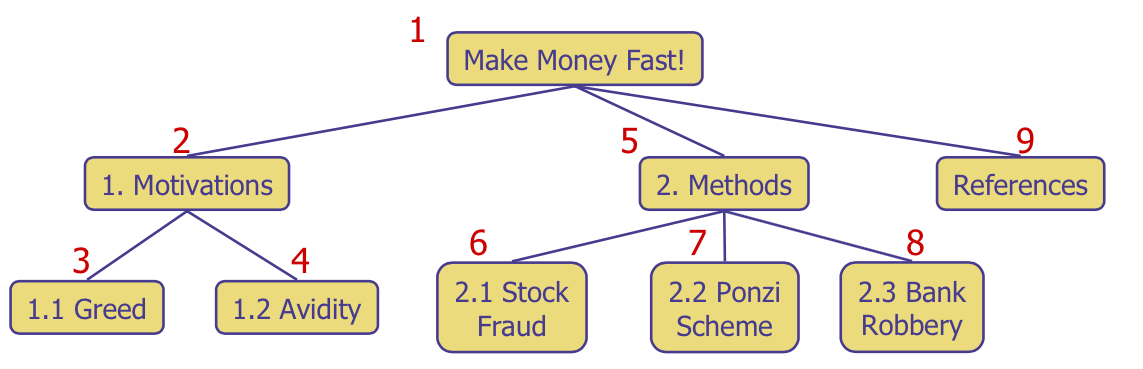
\includegraphics[width=0.8\textwidth]{img/preorder.png}
	\end{center}
\end{figure}
\noindent
Postorder Traversal
\begin{figure}[H]
	\begin{center}
  		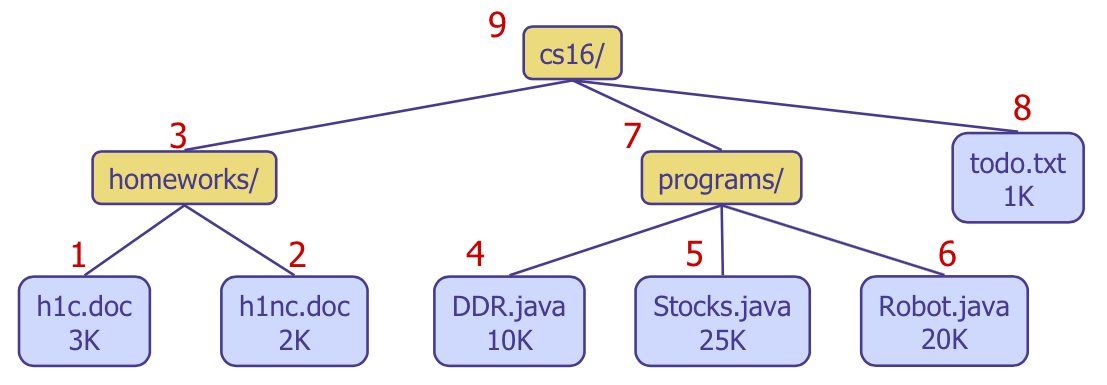
\includegraphics[width=0.8\textwidth]{img/postorder.png}
	\end{center}
\end{figure}
\newpage
%----- Red Black Tree -----%
\subsection{Red Black Tree}
Ein Red Black Tree hat 5 Eigenschaften
\begin{enumerate}
	\item
		Jeder Node ist entweder schwarz oder rot
	\item
		Der root Node ist immer schwarz
	\item
		Jedes child und parent von einem roten Node ist schwarz.\\
		Ein roter Node kann kein rotes Child und keinen roten Parent haben. 
	\item
		Jeder Pfad von Root zu NULL node hat die gleiche Anzahl an schwarzen Nodes.
	\item
		Jedes Leaf ist schwarz
\end{enumerate}
\begin{figure}[H]
	\begin{center}
  		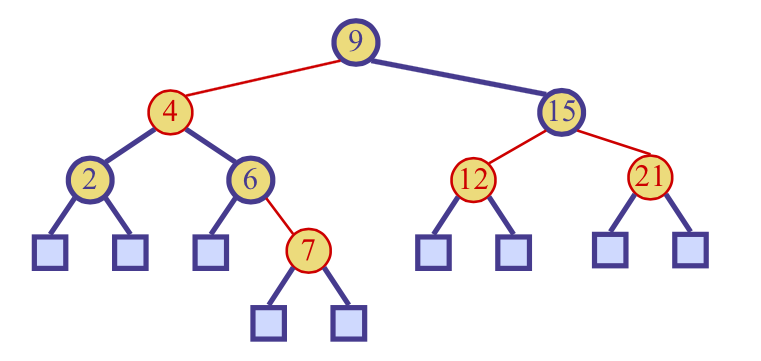
\includegraphics[width=0.8\textwidth]{img/redblack.png}
	\end{center}
\end{figure}
Die meisten BST Operationen (einfügen, suchen, max \ldots) benötigen $O(h)$ Zeit. Wobei $h$ die Höhe des Trees ist. Die Höhe des Red Black Tree ist immer Log n. Damit ist die Laufzeit dieser Operationen in einem Red Black Tree $O(Logn)$.\\
\\
Der Ausgleich des Höhenunterschiedes, wie er beim AVL Tree vorkommt, muss hie rnicht angewendet werden. Ein Red Black Tree ist immer balanciert.  \\
\\
Der Suchalgorithmus in einem Red Bacl Tree ist derselbe wie in einem Binären Suchbaum.
\newpage
\subsubsection{Einfügen}
Die Farbe eines neu eingefügten Elementes ist immer rot.\\
Damit ein solcher Baum nach dem einfügen noch immer in Balance ist, haben wir zwei Mittel.
\begin{enumerate}
	\item
		Recoloring
	\item
		Rotation
\end{enumerate}
Zuerst sollten wir immer Recoloring anzuwenden. Erst dann rotieren wir.\\
\\
z ist das neu eingefügte Element.\\
v ist der parent.\\
w ist der uncle/Sibling des parent. \\
\\
Wir unterscheiden die folgenden Szenarien
\begin{enumerate}
	\item
		Der neu eingefügte Node z wird root. z wird schwarz.
	\item
		Der Parent von z ist schwarz. Wir können den neuen Node einfach anhängen.
	\item
		Der Parent von z ist rot.  Wir haben ein Doppel Rot Problem generiert.
		\begin{figure}[H]
			\begin{center}
  				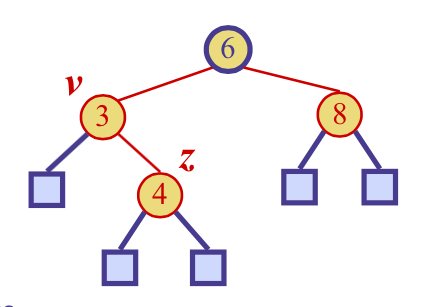
\includegraphics[width=0.6\textwidth]{img/doubleRedIssue.png}
			\end{center}
		\end{figure}
		\newpage
		\textbf{doppel Rot Problematik}\\
		\begin{enumerate}
			\item
			Der Uncle w vom neu eingefügten node z ist Schwarz.\\
			\begin{figure}[H]
				\begin{center}
  					\includegraphics[width=0.4\textwidth]{img/redBlackCase1.png}
				\end{center}
			\end{figure}
			Wir müssen restrukturieren/restructuring durchführen.\\
			\begin{figure}[H]
				\begin{center}
  					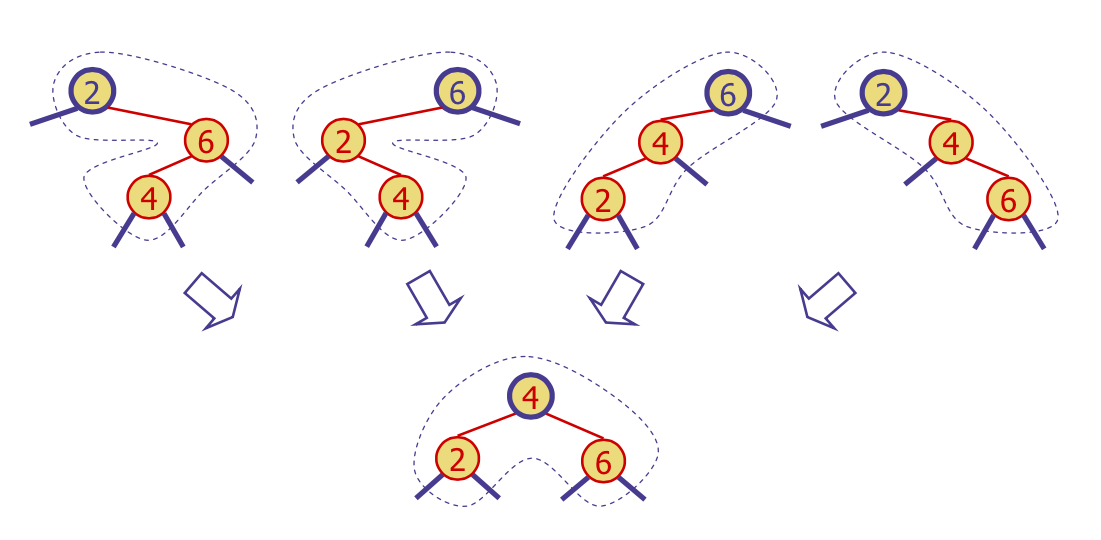
\includegraphics[width=0.8\textwidth]{img/redblackrestructuring.png}
				\end{center}
			\end{figure}
			\newpage
			\textbf{Restructering im Detail}\\
			\\
			Nachfolgend die einzelnen schritte des restrcutering im Detail.\\
			Wir gehen gleich vor wie beim ALV Tree.\\
			\\
			x ist der neu eingefügte Node\\
			p ist der parent.\\
			g ist der grandparent.\\
			u ist der uncle\\
			\begin{itemize}
				\item
				Left Left Case\\
				p ist das linke Kind von g und x ist das linke Kind von p
				\begin{enumerate}
					\item Right Rotation von g
					\item Farbe tauschen von g und p
				\end{enumerate}
				\begin{figure}[H]
					\begin{center}
  						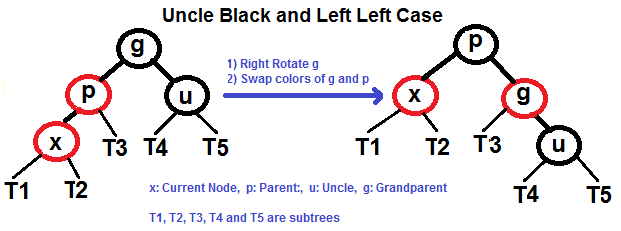
\includegraphics[width=0.8\textwidth]{img/leftleft.png}
					\end{center}
				\end{figure}
				\item
				Left Right Case\\
				p ist das linke Kind von g und x ist das rechte Kind von p
				\begin{figure}[H]
					\begin{center}
  						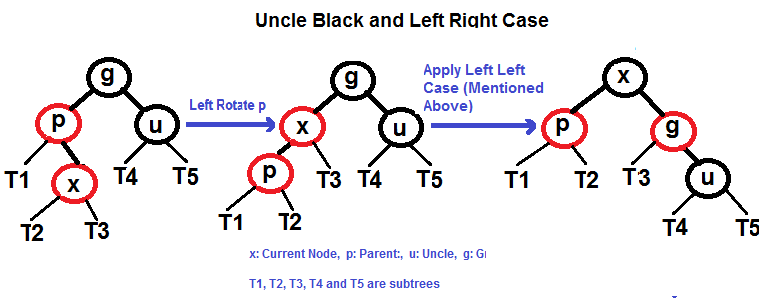
\includegraphics[width=0.8\textwidth]{img/leftright.png}
					\end{center}
				\end{figure}
				\newpage
				\item
				Right Right Case
				\begin{enumerate}
					\item Left Rotation von g
					\item Farbe tauschen von g und p
				\end{enumerate}
				\begin{figure}[H]
					\begin{center}
  						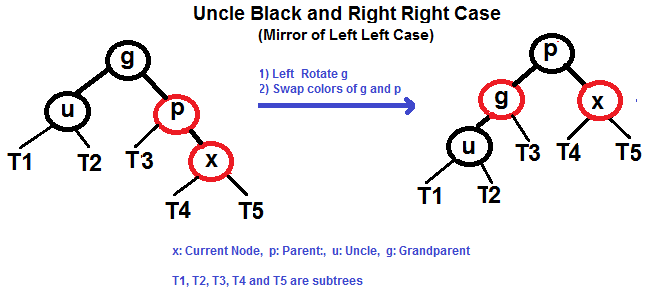
\includegraphics[width=0.8\textwidth]{img/rightright.png}
					\end{center}
				\end{figure}
				\item
				Right Left Case	
				\begin{figure}[H]
					\begin{center}
  						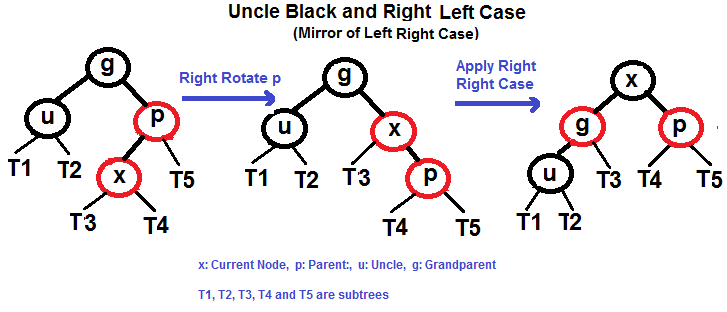
\includegraphics[width=0.8\textwidth]{img/rightleft.png}
					\end{center}
				\end{figure}
				\newpage
			\end{itemize}
			\item
			Der Uncle w von z ist rot
			\begin{figure}[H]
				\begin{center}
  					\includegraphics[width=0.4\textwidth]{img/redBlackCase2.png}
				\end{center}
			\end{figure}
			Wir müssen recolering durchführen.
			\begin{enumerate}
				\item
				Parent v und Uncle w werden Schwarz
				\item
				Grandparent wird Rot, ausser er ist der root knoten
			\end{enumerate}
			\begin{figure}[H]
				\begin{center}
  					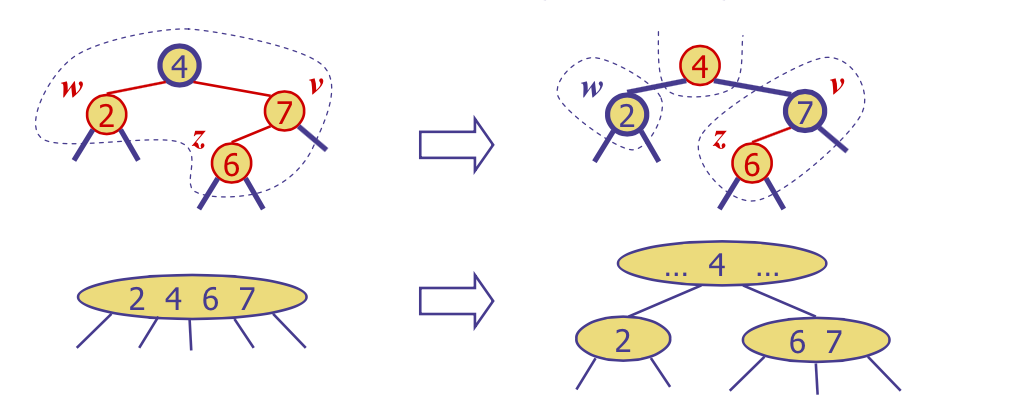
\includegraphics[width=0.8\textwidth]{img/redblackrecoloring.png}
				\end{center}
			\end{figure}
		\end{enumerate}		
\end{enumerate}
\newpage
\subsubsection{Löschen}
v ist das zu löschende interne Element.\\
w ist das zu löschende externe Element. Ist der Sibling von r. child von v. \\
r ist das child von v.
\begin{figure}[H]
	\begin{center}
  		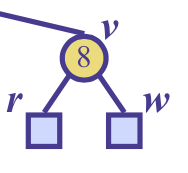
\includegraphics[width=0.35\textwidth]{img/redblackdeletestructure.png}
	\end{center}
\end{figure}
Wir unterscheiden diese Szenarien
\begin{enumerate}
	\item
		Wenn wir den root Knoten löschen wollen.\\
		Wir ersetzen den Root Knoten mit dem ersten inorder Element des rechten Subtrees (analog 2,4 Tree).
	\item
	wenn r oder v rot sind, färben wir r schwarz und löschen den node v.
	\item
	r und v sind beide schwarz. wir färben r double black/ doppel schwarz. Damit ist sind die Bedingungen für einen RotSchwarz Baum nicht mehr erfüllt. Wir müssen den Baum reorganisieren.
\begin{figure}[H]
	\begin{center}
  		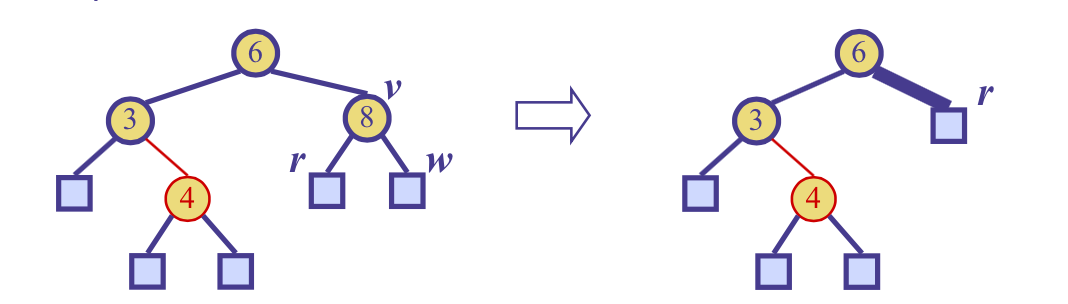
\includegraphics[width=\textwidth]{img/redblackdoubleblack.png}
	\end{center}
\end{figure}
	\newpage
	\textbf{doppel Schwarz Problematik}\\
	\\
	Das doppel Schwarz Problem lässt sich wie folgt lösen
	\begin{enumerate}	
		\item
			y ist schwarz und hat ein rotes Kind\\
			\\
			Wir führen ein restructering durch\\
			\\
			Es gibt 4 Szenarien\\
			\\
			\textbf{Restructuring im Detail}
			\begin{itemize}
				\item
				Left Left\\
				Spiegelung von Right Right
				\item
				Left Right\\
				Spiegelung von Right Left
				\item
				Right Right
				\begin{figure}[H]
					\begin{center}
  						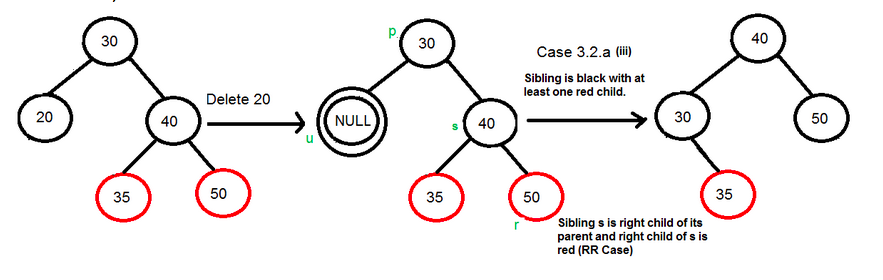
\includegraphics[width=\textwidth]{img/doubleblackdeleteRR.png}
					\end{center}
				\end{figure}
				\newpage
				\item
				Right Left
				\begin{figure}[H]
					\begin{center}
  						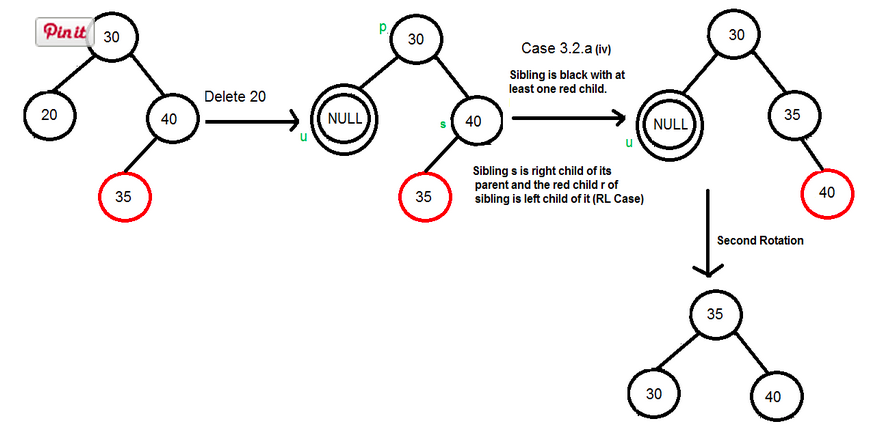
\includegraphics[width=\textwidth]{img/doubleblackdeleteRL.png}
					\end{center}
				\end{figure}
			\end{itemize}
		\newpage
		\item
			y ist schwarz und beide Kinder sind schwarz\\
			\\
			Wir führen ein recoloring durch
			\begin{figure}[H]
				\begin{center}
  					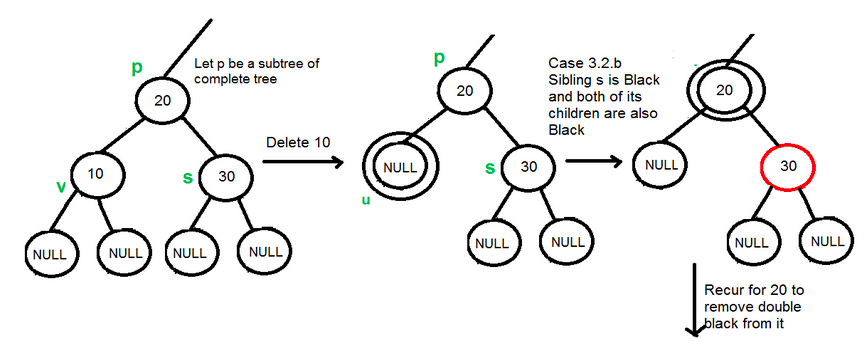
\includegraphics[width=\textwidth]{img/doubleblackdeletionB.png}
				\end{center}
			\end{figure}
			In diesem Beispiel ist der parent node schwarz.\\
			Wenn der parent node rot ist, wird aus dem roten parent ein single black node. (red + double black = single black). Der sibling 35 wird rot.
			\begin{figure}[H]
				\begin{center}
  					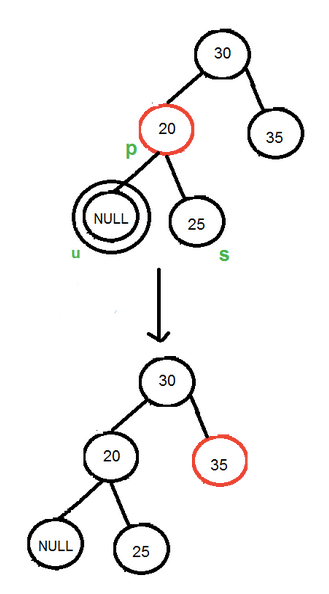
\includegraphics[width=0.3\textwidth]{img/doubleblackdeleteB2.png}
				\end{center}
			\end{figure}
		\newpage
		\item
			y ist rot\\
			\\
			Wir führen Rotationen durch um den alten sibling  nach oben zu bringen
			\begin{itemize}
				\item
					Left Case\\
					Spiegelung von Right Case\\
					Right rotation parent p 
				\item
					Right Case\\
					Left rotation von parent p
					\begin{figure}[H]
						\begin{center}
  							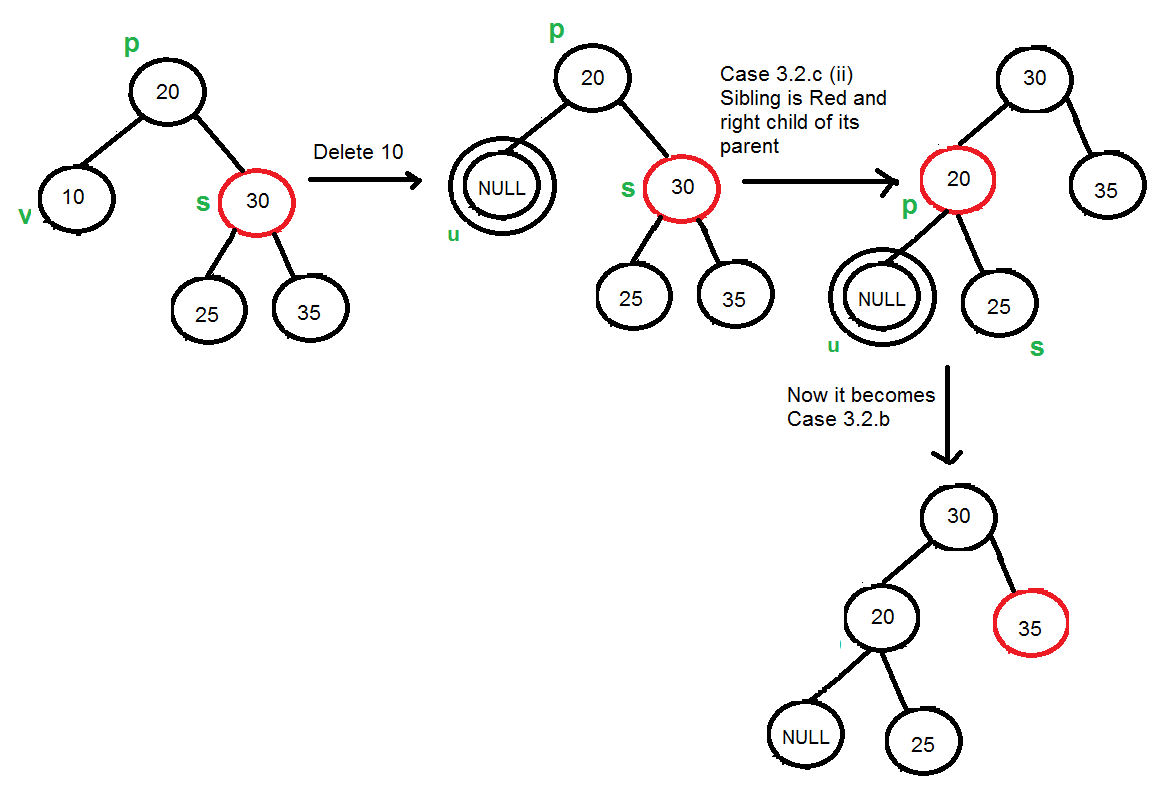
\includegraphics[width=\textwidth]{img/doubleblackdeleteC.png}
						\end{center}
					\end{figure}
			\end{itemize}
		\item
			Wenn r root wird, mach es single black (Die Black height des baumes wird um 1 reduziert).
	\end{enumerate}
\end{enumerate}
\newpage
%----- Splay Tree -----%
\subsection{Splay Tree}
Ein Splay Tree ist nicht balanciert.\\
Dies Grundfunktion eines solchen Baumes ist die Suche.\\
Die Suchfunktion wird solange ausgeführt, bis der gesuchte Node an der Root Position steht.\\
\\
Für die Beispiele wird die nachfolgende Notation verwendet.
\begin{itemize}
	\item
		X ist der Node/ Wert den wir suchen
	\item
		G ist der Parent Node von X
	\item
		P ist der Grossvater Node von X
\end{itemize}
Wir unterscheiden die folgenden Sitiuationen
\newpage
\subsubsection{Zig-Zig}
\begin{itemize}
	\item
		X ist das rechte Kind von P und P ist das rechte Kind von G
		\begin{figure}[h]
			\begin{center}
  			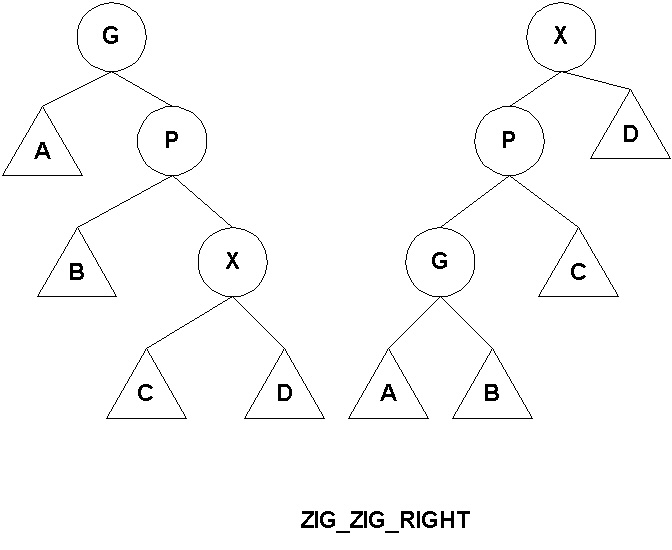
\includegraphics[width=0.5\textwidth]{img/zzright.jpg}
		\end{center}
	\end{figure}
	\item	
		X ist das Linke Kind von P und P ist das linke Kind von G
		\begin{figure}[h]
			\begin{center}
  				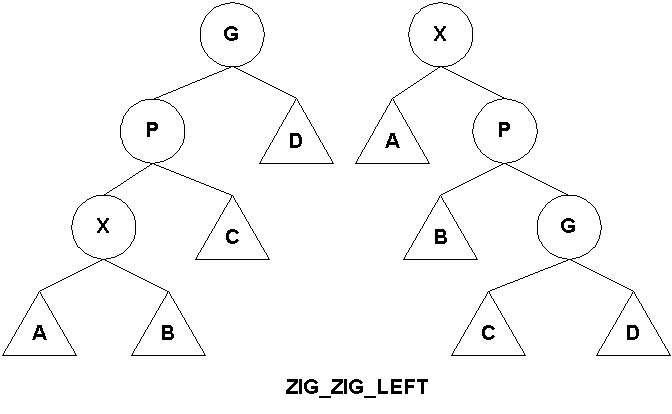
\includegraphics[width=0.5\textwidth]{img/zzleft.jpg}
			\end{center}
		\end{figure}
\end{itemize}
Lösung:
\begin{enumerate}
	\item
		G mit X ersetzen
	\item
		P wird Kind von X
	\item
		G wird Kind von P
\end{enumerate}
\newpage
\subsubsection{Zig-Zag}
\begin{itemize}
	\item
		Wenn P ein linkes und X ein rechtes Kind ist.
		\begin{figure}[h]
			\begin{center}
  			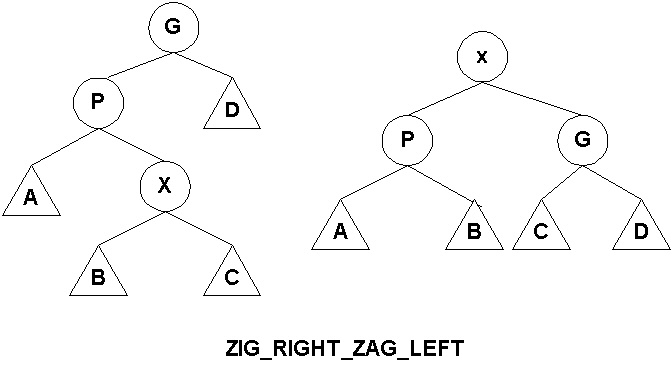
\includegraphics[width=0.5\textwidth]{img/zigRzagL.jpg}
		\end{center}
	\end{figure}
	\item
		Wenn X ein linkes und P ein rechtes Kind ist.
		\begin{figure}[h]
			\begin{center}
  			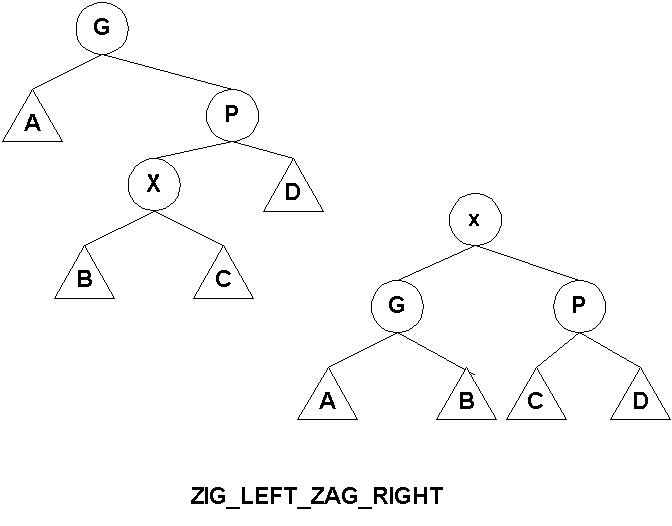
\includegraphics[width=0.5\textwidth]{img/zigLzagR.jpg}
		\end{center}
	\end{figure}
\end{itemize}
Lösung:
\begin{enumerate}
	\item
		G mit X ersetzen
	\item
		G und Z werden Kinder von X. \\Z sollte dabei immer auf der Rechten Seite stehen, da es grösser als X ist.
\end{enumerate}
\newpage
\subsubsection{Zig}
\begin{itemize}
	\item
		X hat keinen Grossvater. X ist ein linkes Kind.
		\begin{figure}[h]
			\begin{center}
  			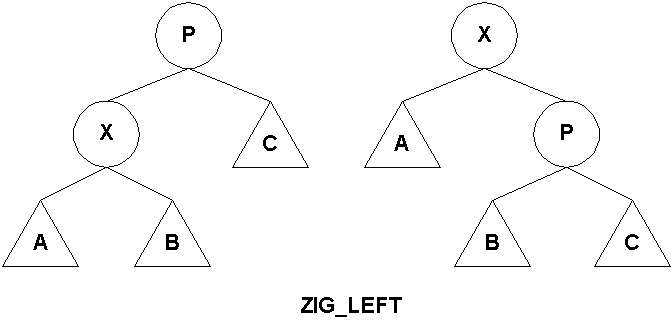
\includegraphics[width=0.5\textwidth]{img/zigleft.jpg}
		\end{center}
	\end{figure}
	\item
		X hat keinen Grossvater. X ist ein rechtes Kind.
		\begin{figure}[h]
			\begin{center}
  			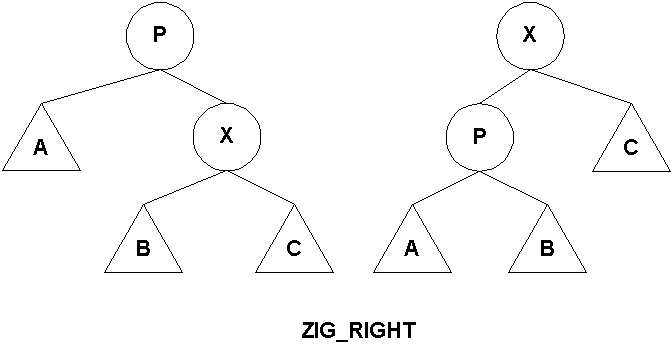
\includegraphics[width=0.5\textwidth]{img/zigright.jpg}
		\end{center}
	\end{figure}
\end{itemize}
Lösung:
\begin{enumerate}
	\item
		X wird mit P getauscht.
	\item
		P wird ein Kind von X. \\
		Eines der früheren Kinder von X bleibt beim X.
\end{enumerate}
\newpage
%----- AVL Tree -----%
\subsection{AVL Tree}
Die Subbäume des AVL Trees dürfen maximal einen Höhenunterschied von 1 haben.\\
AVL Bäume sind immer balanciert.\\
\\
Ist ein Binary Search Tree.
\begin{figure}[H]
	\begin{center}
  		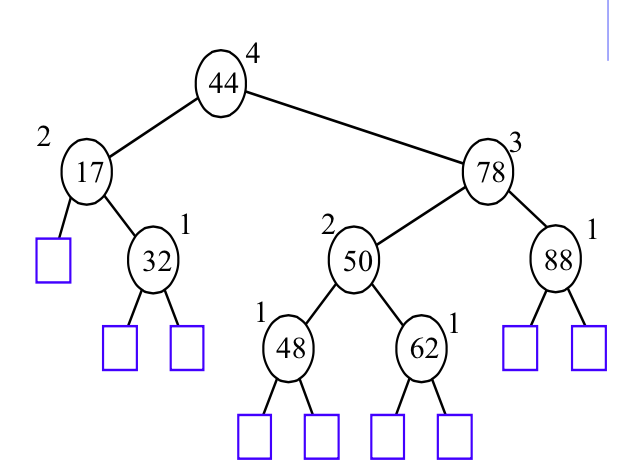
\includegraphics[width=0.6\textwidth]{img/avltree.png}
	\end{center}
\end{figure}
\noindent
Die Höhe eines AVL Tree ist $O(log n)$, wobei n die Anzahl gespeicherten Elemente ist.
\subsubsection{Einfügen}
Wir wollen 54 einfügen.\\
Wir hängen das neue Element immer an einen externen Node. 
\begin{figure}[H]
	\begin{center}
  		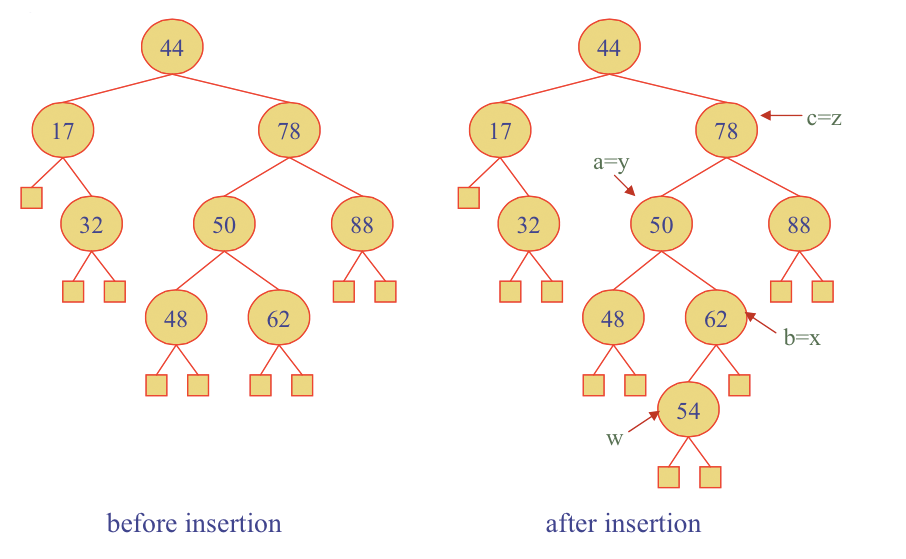
\includegraphics[width=0.6\textwidth]{img/avltreeinsertion.png}
	\end{center}
\end{figure}
\noindent
Nun ist aber für den Node 78 der Höhenunterschied seiner Äste auf 2 angestiegen.\\
Der Baum ist nicht mehr balanciert.\\
Wir müssen den Baum restrukturieren.
\subsubsection{Restructering}
\begin{figure}[H]
	\begin{center}
  		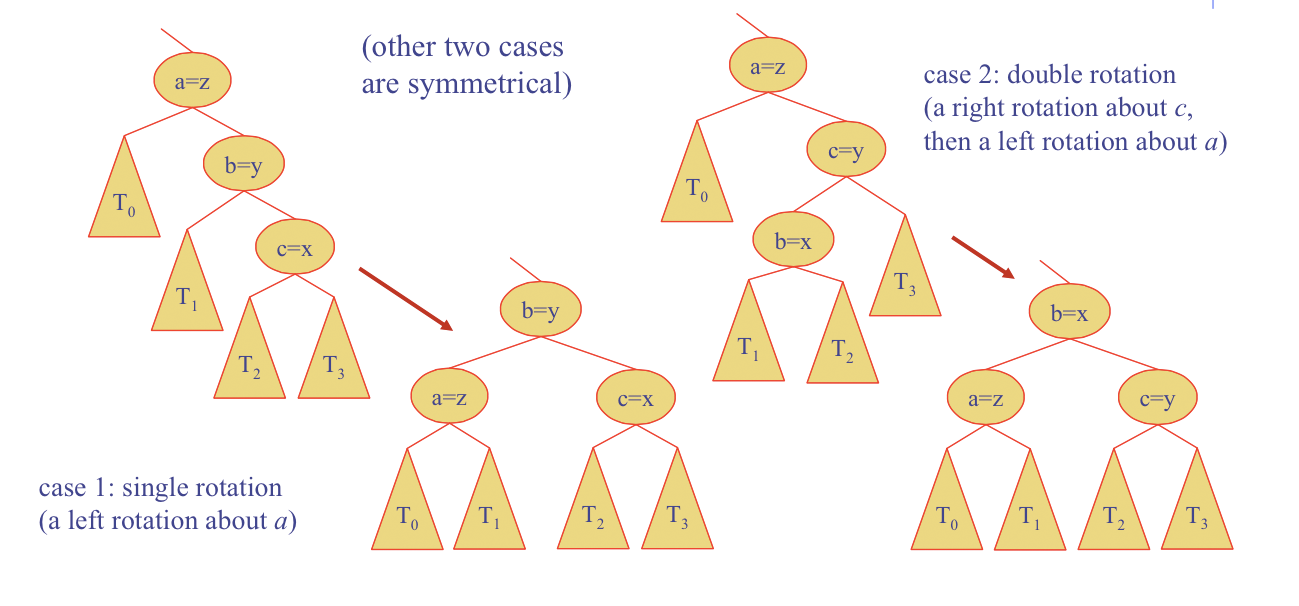
\includegraphics[width=\textwidth]{img/avltreerestructering.png}
	\end{center}
\end{figure}
\subsubsection{Treerotation}
\textbf{Single Rotation}\\
\begin{figure}[H]
	\begin{center}
  		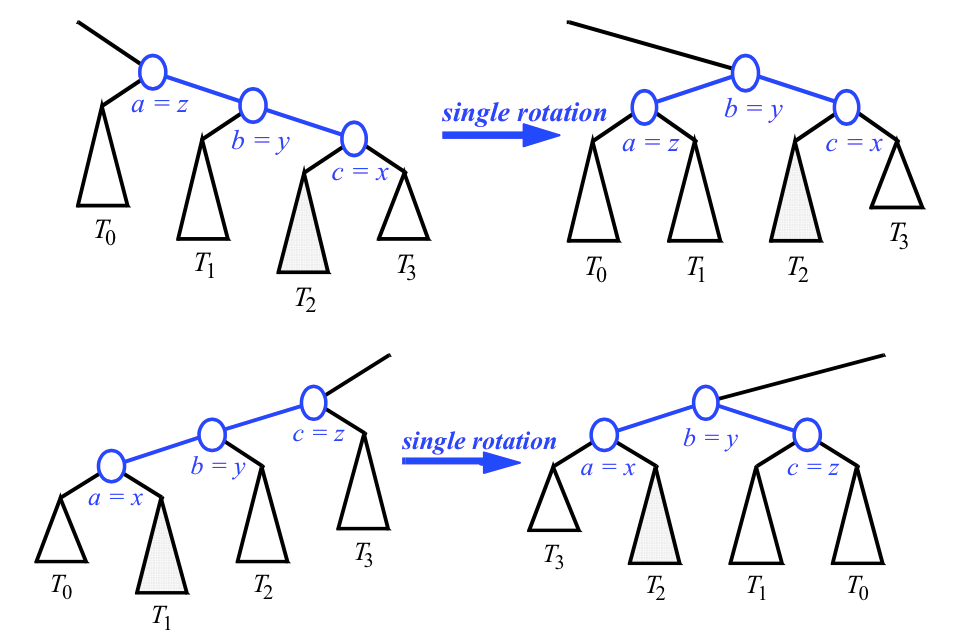
\includegraphics[width=\textwidth]{img/singlerotation.png}
	\end{center}
\end{figure}
\noindent
\textbf{Left Rotation}\\
Es Passieren 3 Operationen
\begin{enumerate}
	\item 
		Wir merken uns den rechten Sub Tree
	\item
		Der linke Subtree des neuen Roots wird dem alten Root rechts angehängt		
	\item
		Der alte Root wird dem neuen Root links angehängt
\end{enumerate}
\begin{lstlisting}
function LeftRotation(node)
{
	/* Predfinition: node.Left ! == null
	Post: node.Left is the new root of the subtree, node has become node.Left s right child and, BST properties are preserved */

	node newRoot = node.Right;
	node.right = newRoot.Left;
	newRoot.Left = node;
}
\end{lstlisting}
\textbf{Right Rotation}\\
Es Passieren 3 Operationen
\begin{enumerate}
	\item 
		Wir merken uns den linke Sub Tree
	\item
		Der rechte Subtree des neuen Roots wird dem alten Root links angehängt		
	\item
		Der alte Root wird dem neuen Root rechts angehängt
\end{enumerate}
\begin{lstlisting}
function RightRotation(node)
{
	/* Predfinition: node.Left ! == null
	Post: node.Left is the new root of the subtree, node has become node.Left s right child and, BST properties are preserved */

	node newRoot = node.Left;
	node.left = newRoot.Right;
	newRoot.Right = node;
}
\end{lstlisting}
\newpage
\textbf{Double Rotation}
\begin{figure}[H]
	\begin{center}
  		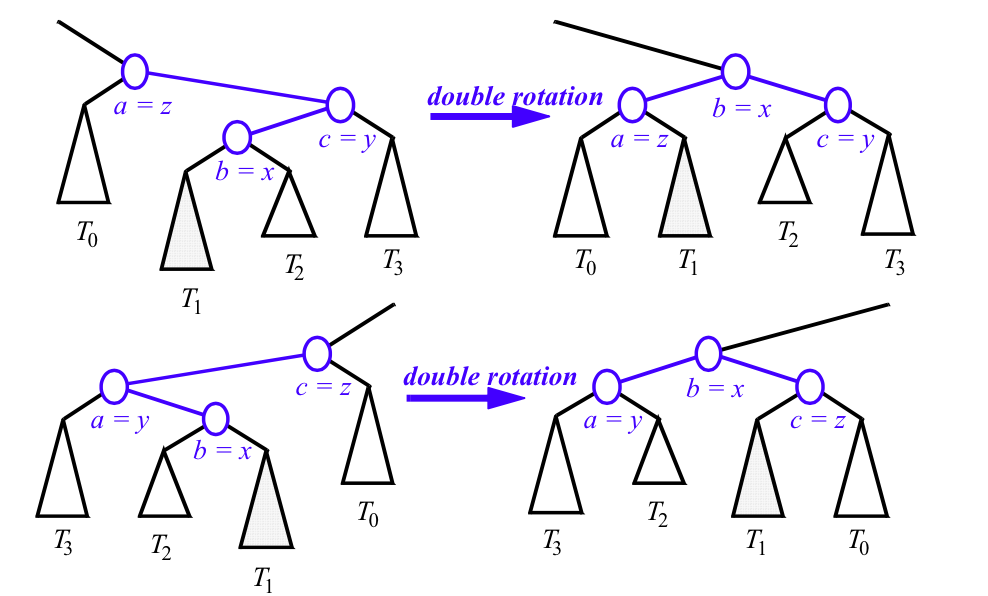
\includegraphics[width=0.9\textwidth]{img/doublerotation.png}
	\end{center}
\end{figure}
\textbf{Rotation Example}
\begin{figure}[H]
	\begin{center}
  		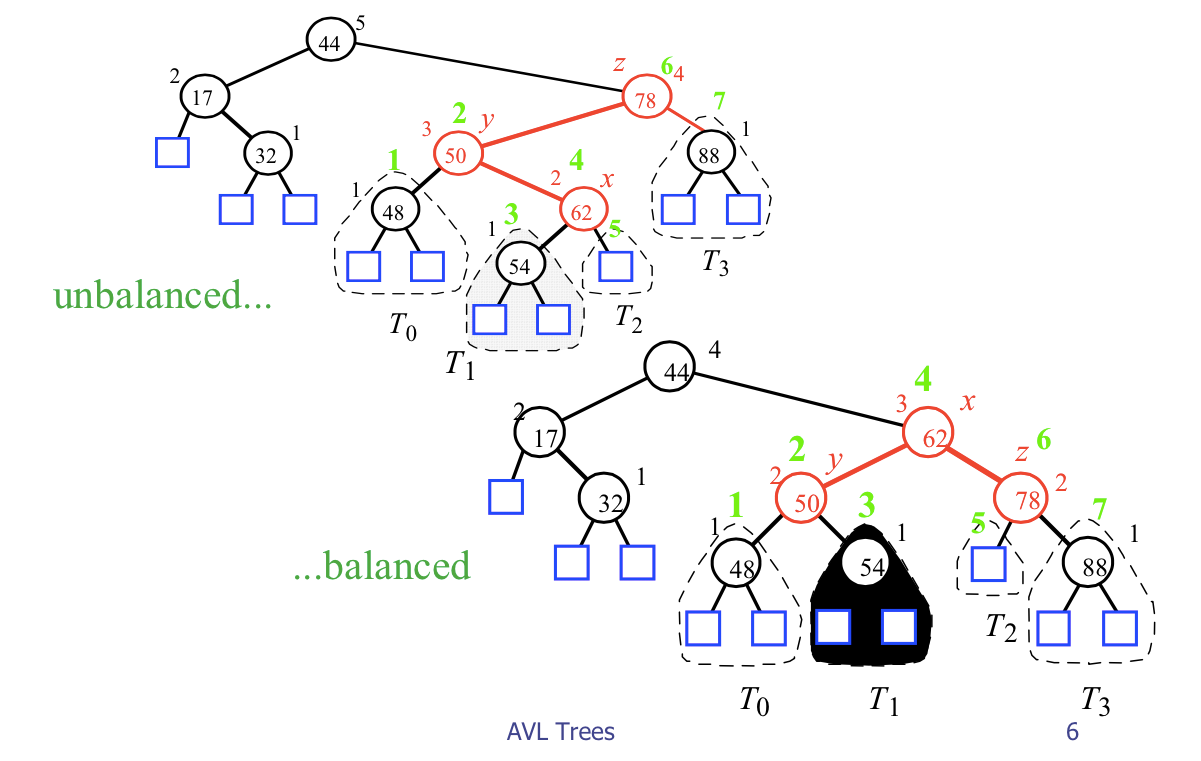
\includegraphics[width=0.9\textwidth]{img/rotationexample.png}
	\end{center}
\end{figure}
\newpage
\subsubsection{Löschen}
Der gelöschte Node wird ein leerer externer Node des parent.\\
Gleiches vorgehen wie beim Binary Seach Tree.
\begin{figure}[H]
	\begin{center}
  		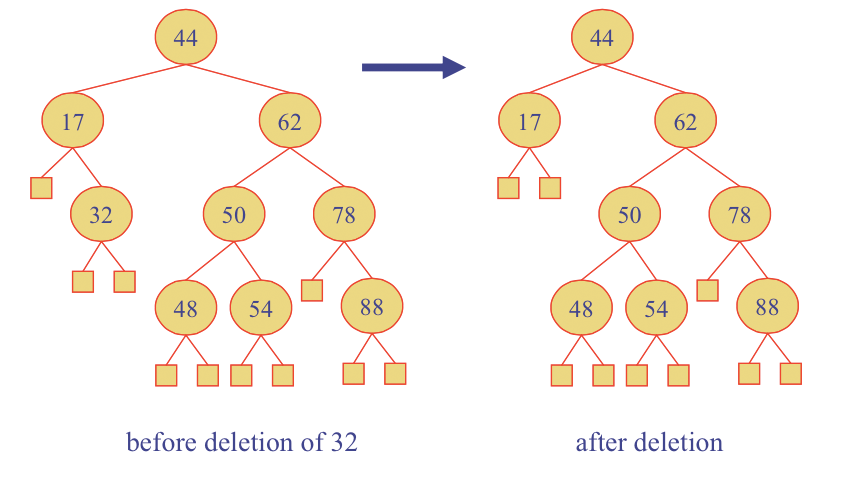
\includegraphics[width=0.9\textwidth]{img/avltreedeletion.png}
	\end{center}
\end{figure}
\newpage
%----- Binary Search Tree -----%
\subsection{Binary Search Tree}
Jeder Binäre Suchbaum besitz ein Node Element/ Root mit dem Wert x. Der Linke Subtree von Root beinhaltet alle Elemente die kleiner sind als x, < x. Der Rechte Subtree beinhaltet alle Elemente die grösser gleich als x sind, \underline{>} x.
\begin{figure}[H]
\begin{center}
  	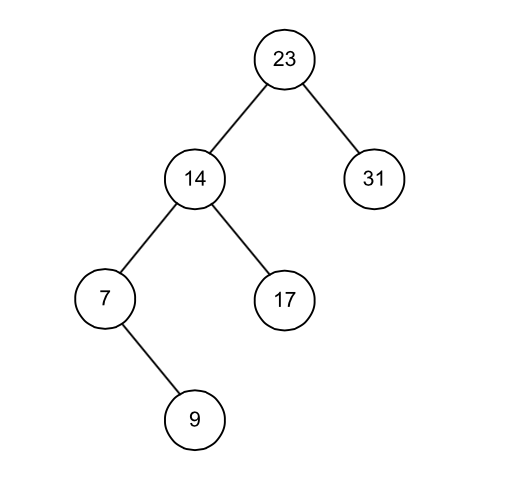
\includegraphics[width=0.5\textwidth]{img/binarysearchtree.png}
	\caption{Einfacher unabalancierter binäre Suchbaum}
\end{center}
\end{figure}
Inorder Traversal
\begin{figure}[H]
	\begin{center}
  		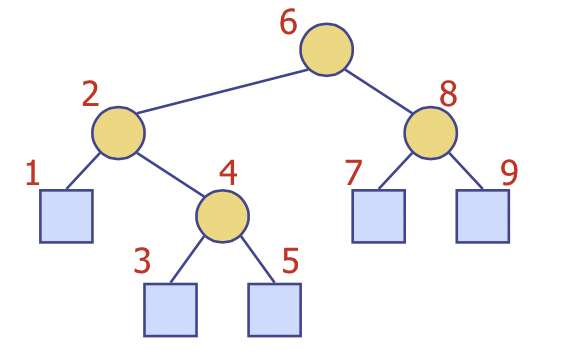
\includegraphics[width=0.6\textwidth]{img/bstinorder.png}
	\end{center}
\end{figure}
\newpage
\subsubsection{Einfügen}
Der Aufruf funktioniert rekursiv.\\
\\
Code:
\begin{lstlisting}
// Check if root is available
function Insert(value)
{
	if (root == null) // No root exists 
	{
		root =  new node(value) ;
	}
	else
	{
		InsertNode(root, value);
	}
}

function InsertNode(current, value)
	// check size
	if(value < current.Value)
	{
	// Smaller, value will be added left
		if(current.Left ==  null)
		{
			current.Left  = new node(value);
		}
		else
		{
			InsertNode(current.Left, value);
		}
	}
	else
	// Bigger as root, value will be added right
	{
		if(current.Right == null)
		{
			current.Right = new node(value);
		}
		else
		{
			InsertNode(current.Right, value)
		}
	}
\end{lstlisting}
\newpage
\subsubsection{Suchen}
Es gibt 4 Szenarien, die wir unterschieden müssen.
\begin{enumerate}
	\item the root == null in which case value is not in the BST
	\item root.Value == value in which case value is in the BST
	\item value < root.Value, we must inspect the left subtree of root for value
	\item value > root.Value, we must inspect the right subtree of root for value
\end{enumerate}
\begin{lstlisting}
functions contains(root, value)
{
	if(root == null)
	{
		return false
	}
	if(root.Value == value)
	{
		return true;
	}
	else if(value < root.Value)
	{
		contains(root.left, value);
	}
	else
	{
		contains(root.right, value);
	}
}
\end{lstlisting}
\newpage
\subsubsection{Löschen}
Es gibt 4 Szenarien, die wir unterschieden müssen.\\
\begin{enumerate}
	\item the value to remove is a leaf node\\
	just remove the node
	\item the value to remove has a right subtree, but no left subtree\\
	We link the parent with the right subtree
	\item the value to remove has a left subtree, but no right subtree\\
	We link the parent with the left subtree
	\item the value to remove has both a left and right subtree\\
	we promote the largest value in the left subtree
\end{enumerate}
\newpage
\subsubsection{Arithmetic Expression Tree} 
Interne Nodes sind Operatorem\\
Externe Nodes sind Zahlen/ Variabeln
\begin{equation*}(2*(a-1)+(3*b))\end{equation*}
\begin{figure}[H]
	\begin{center}
  		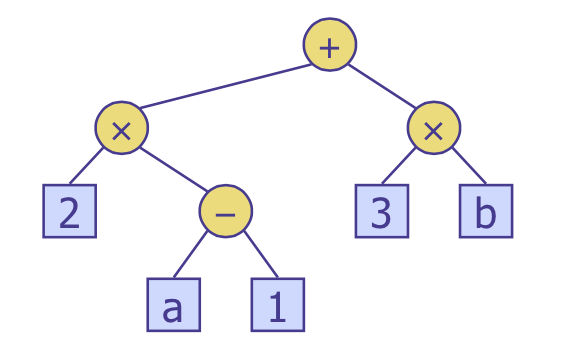
\includegraphics[width=0.7\textwidth]{img/arithmeticexpression.png}
	\end{center}
\end{figure}
\subsubsection{Decision Tree}
Enstcheidung wo man essen gehen will
\begin{figure}[H]
	\begin{center}
  		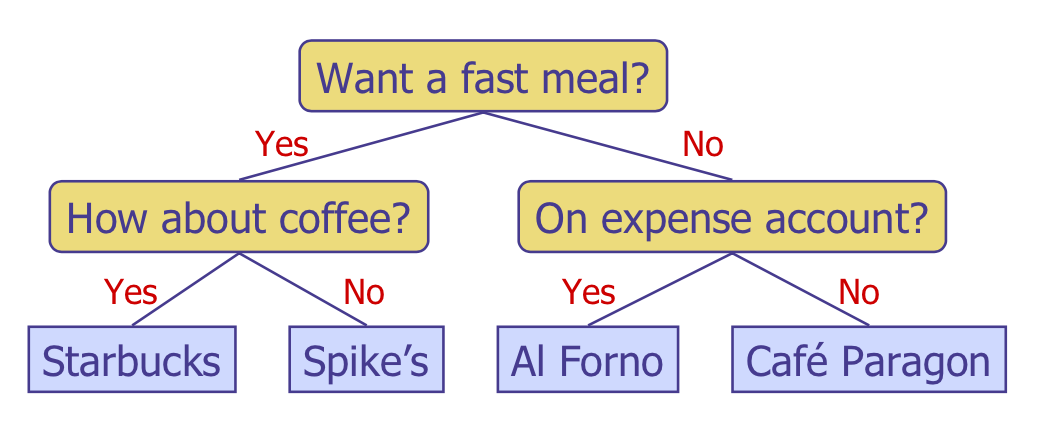
\includegraphics[width=0.7\textwidth]{img/decisiontree.png}
	\end{center}
\end{figure}
\newpage
\subsection{Multi-Way Search Tree}
Eigenschaften:
\begin{itemize}
	\item
	Die Leafs dienen nur als Platzhalter.
	\item
	Jeder Interne Knoten besitzt mindestens 2 Kinder und speichert d-1 Key Items.\\
	Wobei d die Anzahl der Kinder ist.
\end{itemize}
\begin{figure}[H]
	\begin{center}
  		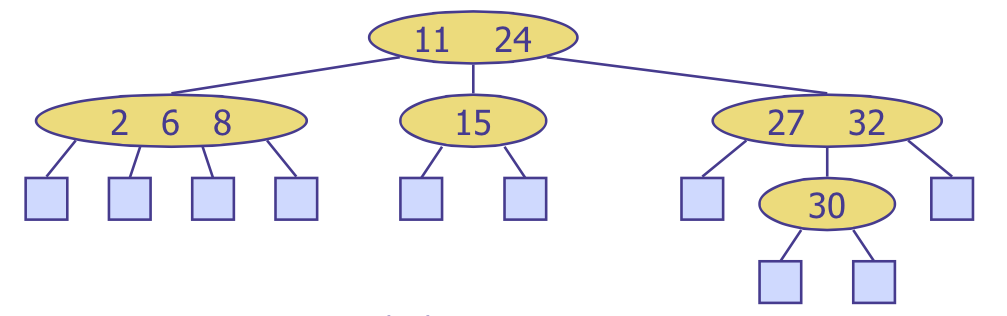
\includegraphics[width=0.9\textwidth]{img/multiwaysearchtree.png}
	\end{center}
\end{figure}
\subsubsection{Searching}
Inorder Traversal\\
\\ 
Eine Inorder Traversierung besucht die Keys in aufsteigender Reihenfolge.
\begin{figure}[H]
	\begin{center}
  		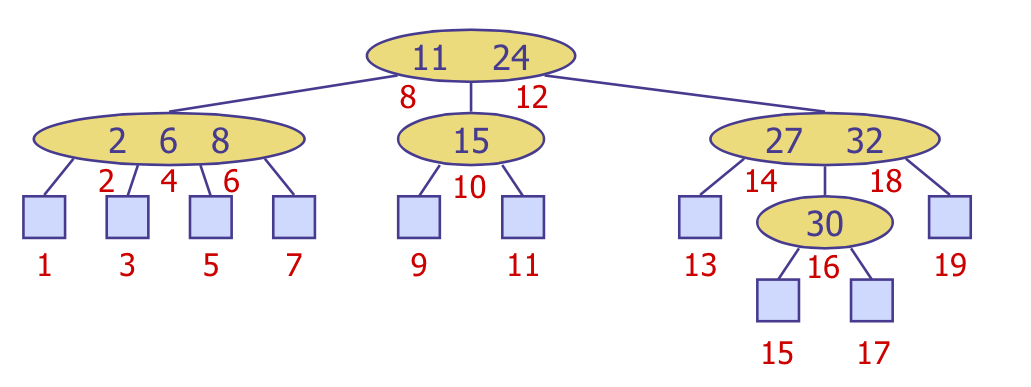
\includegraphics[width=0.9\textwidth]{img/multiwaysearchtreeinorder.png}
	\end{center}
\end{figure}
\newpage
\subsection{2,4 Tree}
Auch 2-4 tree oder 2,3,4 Tree genannt.\\
Ist ein Multiway Search Tree.\\
\\
Eigenschaften:
\begin{itemize}
	\item
		Jeder interne Knote hat maxima 4 Kinder
	\item
		Jeder Externe Knoten hat die selbe Tiefe
\end{itemize}
Ein 2,4 Tree mit n elementen hat die Höhe $O(log n)$\\
Die Suche in einem 2,4 Tree dauert $O(log n)$
\begin{figure}[H]
	\begin{center}
  		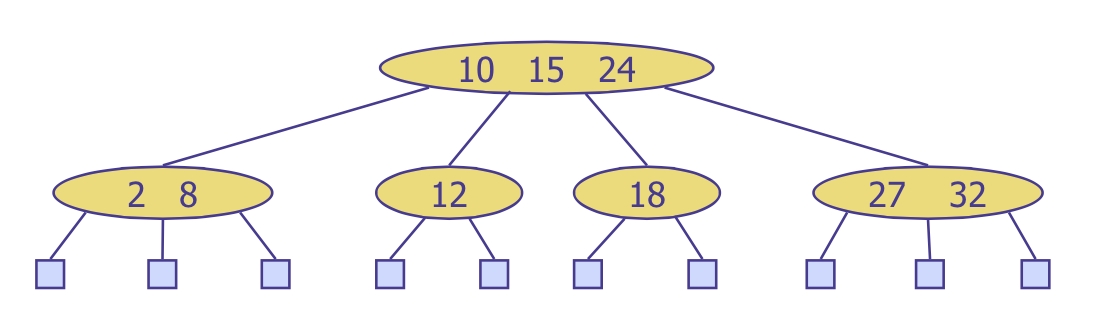
\includegraphics[width=0.8\textwidth]{img/24tree.png}
	\end{center}
\end{figure}
\noindent
Um sich das ganze besser vorstellen zu können, hilft es sich den 2,4 Baum als Red Black Tree aufzuzeichnen.
\newpage
\subsubsection{Einfügen}
Wir wollen den Key 30 einfügen.\\
Wir fügen 30 zum Knoten v hinzu.\\
Wir generieren einen Overflow, da ein interner Knoten max 4 Kinder haben darf.
\begin{figure}[H]
	\begin{center}
  		\includegraphics[width=0.9\textwidth]{img/24treeinsertion1.png}
	\end{center}
\end{figure}
\noindent
Wir führen einen Split durch. Node v wird augeteilt.\\
Key 32 wird zum Parent hinzugefügt.\\
v': 27 und 30 bilden einen 3-Node.\\
v'': 35 bildet einen 2-Node
\begin{figure}[H]
	\begin{center}
  		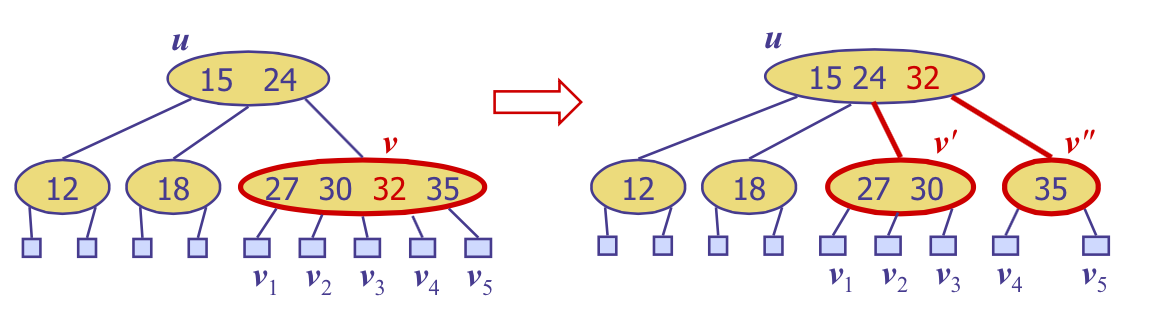
\includegraphics[width=0.9\textwidth]{img/24treeinsertion2.png}
	\end{center}
\end{figure}
\newpage
\subsubsection{Löschen}
Wir wollen Key 24. löschen \\
Wir ersetzen 24 mit dem 1. inorder Element (inorder Successor) des rechte Knotens.\\
In diesem Fall 27.
\begin{figure}[H]
	\begin{center}
  		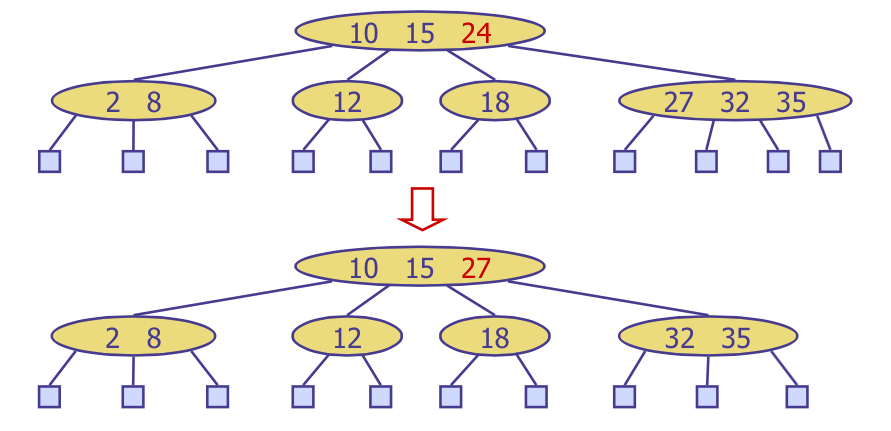
\includegraphics[width=0.9\textwidth]{img/24treedeletion1.png}
	\end{center}
\end{figure}
\newpage
\noindent
\textbf{Underflow}\\
Wenn wir Elemente aus einem 2,4 Tree löschen, kann es zu einem Underflow kommen.\\
Node v wird in diesemfalle ein 1-Node mit nur einem Kind und keinem Key.\\
\\
w: sibling\\
u: parent\\
v: underflown node
\\
\\
Es gibt 2 Möglichkeiten einen Underflow zu beheben
\begin{enumerate}
	\item
		Fusion:\\
		\\
		Wir fusionieren w mit v. Es entsteht der Knoten v'.\\ 
		Wir transferien einen Key von u nach v'.\\
		\\
		Achtung. Eine Fusion kann zu einem Underflow im parent u führen
		\begin{figure}[H]
			\begin{center}
  				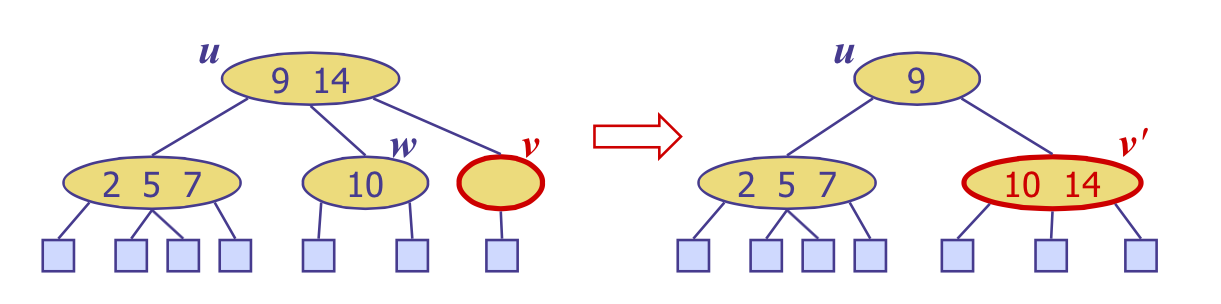
\includegraphics[width=0.9\textwidth]{img/underflow1.png}
			\end{center}
		\end{figure}
	\item
		Transfer:\\
		\\
		Wenn der sibling w ein 3 oder 4-Node ist, können wir einen Transfer durchführen.\\
		\\
		1.) Wir verschieben ein Child von w nach v\\
		2.) Wir verschieben ein Key von u nach v\\
		3.) Wir verschieben ein Key von w nach u\\
		\\
		Nach einem Transfer sind alle Underflows behoben.
		\begin{figure}[H]
			\begin{center}
  				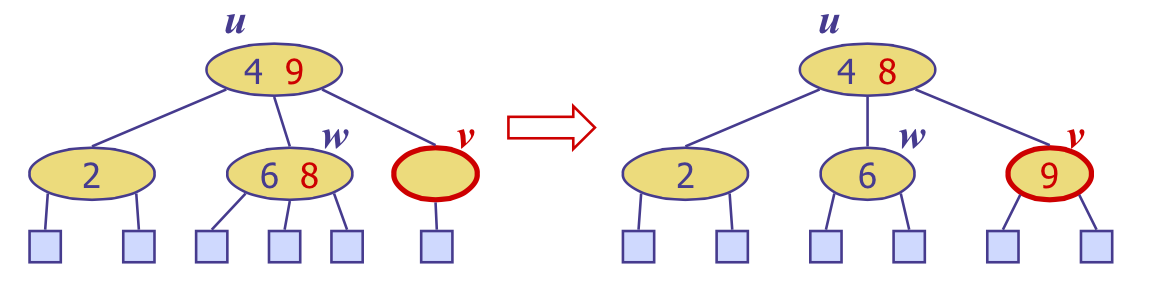
\includegraphics[width=0.9\textwidth]{img/underflow2.png}
			\end{center}
		\end{figure}
\end{enumerate}
\newpage
\subsubsection{2,4 to Red Black Tree}
Ein Red Black Tree kann recht simpel in einen 2,4 Baum umgewandelt werden.\\
Jeder schwarze Node gibt einen neuen Knoten im 2,4 Baum.\\
Die roten Kinder werden in diesen Knoten aufgenommen.
Der schwarze Node steht dabei in der Mitte. Die Kinder 2 und 7 stehen links resp. rechts.
\begin{figure}[H]
	\begin{center}
  		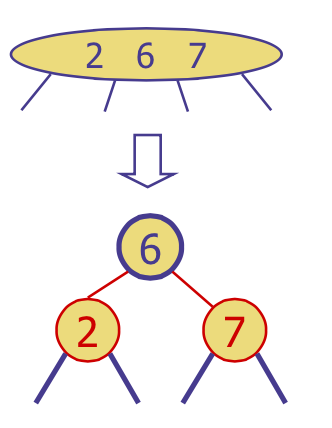
\includegraphics[width=0.3\textwidth]{img/24newNode.png}
	\end{center}
\end{figure}
\noindent
Manche Strukturen lassen sich nicht definitiv bestimmen. 5 wie auch 3 könnten hier der schwarze Node sein.
\begin{figure}[H]
	\begin{center}
  		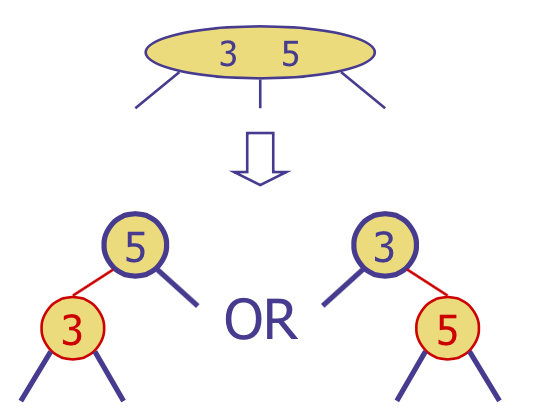
\includegraphics[width=0.5\textwidth]{img/24or.png}
	\end{center}
\end{figure}
\newpage
\section{Graphen}
\subsection{BFS, Breadth-first search}
Java Code:
\begin{lstlisting}
// Not discovered node
private static final int FRESH = 0;
// Open node
private static final int OPEN = 1;
//Closed node
private static final int CLOSED = 2;
/**
 * Breadth-first search
 *
 * @param graph graph to be traversed
 * @param rootNr root node
 * @return array of predecessors
 */
public static GraphNodeIface[] breadthFirstSearch(GraphIface graph, int rootNr) {
    GraphNodeIface[] predecessors = new GraphNodeIface[graph.getVertexCount()]; //array of predecessors
    int[] state = new int[graph.getVertexCount()];
    for (int i = 0; i < state.length; i++) {
        state[i] = FRESH;
    }
    state[rootNr] = OPEN; //root node is open
    predecessors[rootNr] = null; //root has no predecessor

    Queue<GraphNodeIface> l = new LinkedList<GraphNodeIface>(); //queue, by replacing with stack the algorithm would behave as DFS
    l.add(graph.getNode(rootNr));

    while (!l.isEmpty()) {
        GraphNodeIface node = l.poll();
        List<GraphNodeIface> successors = node.getSuccessors();
        for (GraphNodeIface succ : successors) { 
            if (state[succ.getId()] == FRESH) { //newly discovered node
                l.add(succ); //to be processed
                state[succ.getId()] = OPEN;
                predecessors[succ.getId()] = node;
            }
        }
        state[node.getId()] = CLOSED;
    }
    return predecessors;
}
\end{lstlisting}
\newpage
\subsection{DFS, Depth-first search }
Java Code:
\begin{lstlisting}
// Not discovered node
private static final int FRESH = 0;
// Open node
private static final int OPEN = 1;
//Closed node
private static final int CLOSED = 2;
/**
 * Recursive form of depth-first search
 *
 * @param graph
 */
public static void depthFirstSearch(GraphIface graph) {
    //node states
    int[] state = new int[graph.getVertexCount()];

    for (int i = 0; i < state.length; i++) {
        state[i] = FRESH;
    }
    //perform depth first search of all connected components
    for (int i = 0; i < graph.getVertexCount(); i++) {
        if (state[i] == FRESH) {
            doDFS(graph, i, state);
        }
    }
}

/**
 * Perform depth-first search
 *
 * @param graph graph
 * @param vertexNr node identifier
 * @param state array of node states
 */
private static void doDFS(GraphIface graph, int vertexNr, int[] state) {
    state[vertexNr] = OPEN;
    List<GraphNodeIface> succ = graph.getNode(vertexNr).getSuccessors();
    for (GraphNodeIface n : succ) {
        if (state[n.getId()] == FRESH) {
            doDFS(graph, n.getId(), state);
        }
    }
    state[vertexNr] = CLOSED;
}
\end{lstlisting}
\newpage
\subsection{Floyd-Warshall}
Der Floyd-Warshall Algorithmus wird dazu verwendet, den kürzesten/ längsten Pfad  für alle Node Paare, die keinen Cycle order negative Länge enthalten, zu finden.\\
\\
Der Floyd Warshall Algorithmus nutzt eine Matrix $D$ als Input.\\
In dieser Matrix werden die Distanzen/ Verbindungskosten zwischen den einzelnen Nodes vermerkt.\\ Besteht keine direkte Verbindung wird $\infty$ eingetragen.
\begin{figure}[H]
	\begin{center}
  		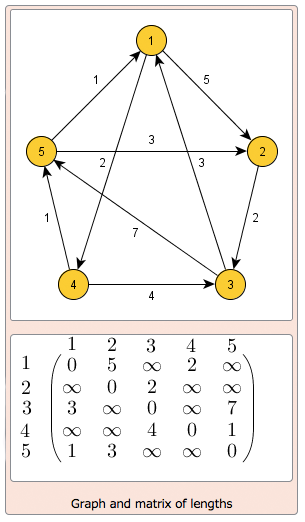
\includegraphics[width=0.5\textwidth]{img/floyd.png}
	\end{center}
\end{figure}
\noindent
Vertikale Achse: Verbindung von\\
Horizontale Achse: Verbindung zu
\newpage
\begin{myexample}
\begin{figure}[H]
	\begin{center}
  		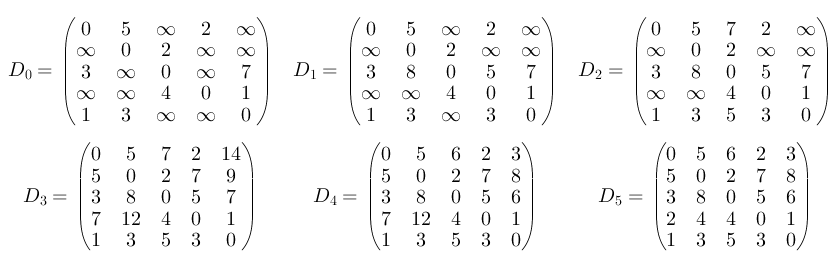
\includegraphics[width=\textwidth]{img/floydexample.png}
	\end{center}
\end{figure}
\begin{enumerate}
	\item
	$D_0$\\
	Die Input Matrix
	\item
	Wir suchen die kürzeste Distanz und tragen Sie in die Matrix ein.
\end{enumerate}
\end{myexample}
\newpage
\noindent
Java Code:
\begin{lstlisting}
/**
 * Floyd-Warshall algorithm. Finds all shortest paths among all pairs of nodes
 * @param d matrix of distances (Integer.MAX_VALUE represents positive infinity)
 * @return matrix of predecessors
 */
public static int[][] floydWarshall(int[][] d) {
    int[][] p = constructInitialMatixOfPredecessors(d);
    for (int k = 0; k < d.length; k++) {
        for (int i = 0; i < d.length; i++) {
            for (int j = 0; j < d.length; j++) {
                if (d[i][k] == Integer.MAX_VALUE || d[k][j] == Integer.MAX_VALUE) {
                    continue;                  
                }
                
                if (d[i][j] > d[i][k] + d[k][j]) {
                    d[i][j] = d[i][k] + d[k][j];
                    p[i][j] = p[k][j];
                }

            }
        }
    }
    return p;
}

/**
 * Constructs matrix P0
 * @param d matrix of lengths
 * @return P0
 */
private static int[][] constructInitialMatixOfPredecessors(int[][] d) {
    int[][] p = new int[d.length][d.length];
    for (int i = 0; i < d.length; i++) {
        for (int j = 0; j < d.length; j++) {
            if (d[i][j] != 0 && d[i][j] != Integer.MAX_VALUE) {
                p[i][j] = i;
            } else {
                p[i][j] = -1;
            }
        }
    }
    return p;
}
\end{lstlisting}
\newpage
\subsection{Minimum Spanning Trees (MST)}
Jedes Element ist untereinander verbunden.\\
Es gibt keine Loops/ Kreisverbindungen.\\
\\
Um einen MST zu bauen, darf bei jedem Element begonnen werden.\\
Wir suchen die Verbindung mit den niedrigesten Verbindungskosten.
\subsubsection{Prim-Jarnik’s}
\begin{myexample}
Start bei \textbf{DFW}. Mit der nächste Verbindung gelangen wir  entweder zu \textbf{DEN} oder \textbf{STL}. Wir wählen die Verbindung zu DEN, da die Verbindungkosten nur bei 4 liegen.\\
Von DEN aus gesehen ist ORD die nächst günstigste Verbindung.\\
usw\ldots
\begin{figure}[H]
	\begin{center}
  		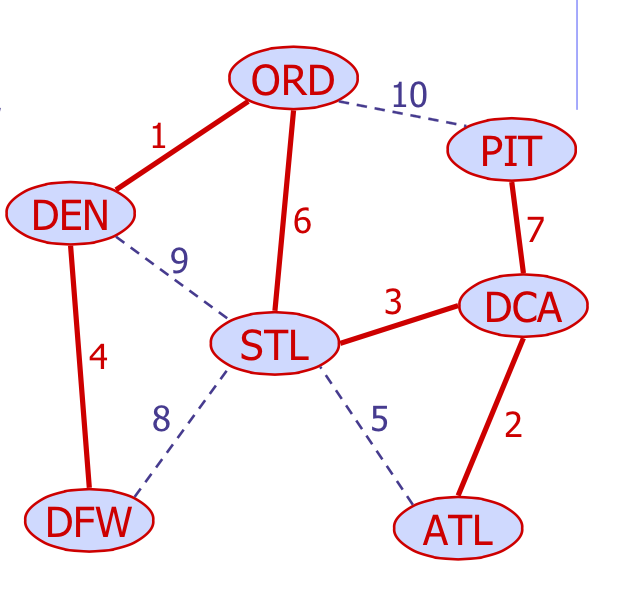
\includegraphics[width=0.8\textwidth]{img/mst.png}
	\end{center}
\end{figure}
\end{myexample}
\newpage
\subsubsection{Kruskal}
Die Ausgangslage
\begin{figure}[H]
	\begin{center}
  		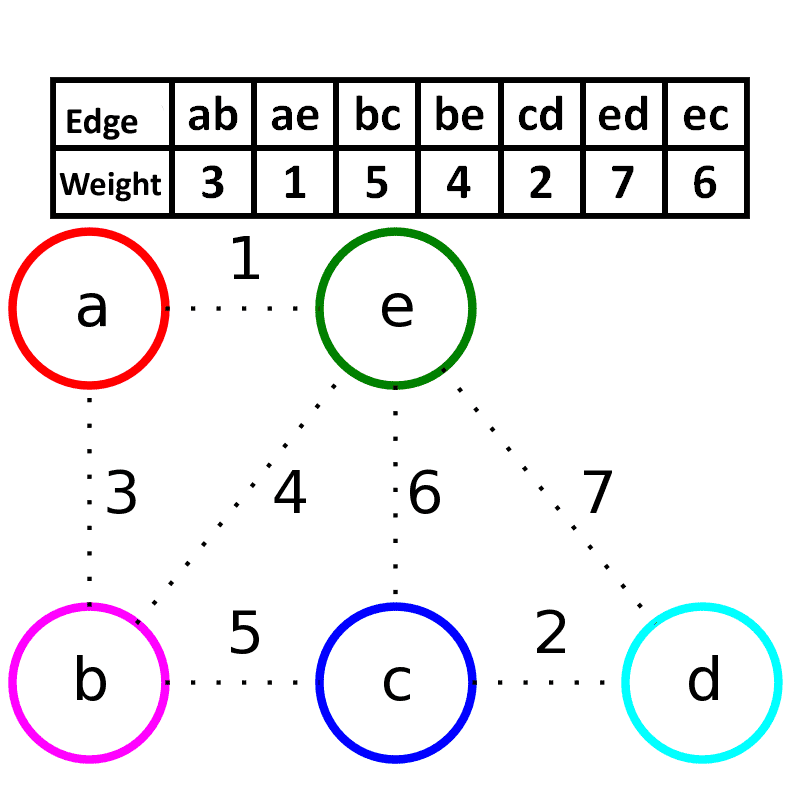
\includegraphics[width=0.4\textwidth]{img/kruskal1.png}
	\end{center}
\end{figure}
\begin{enumerate}	
	\item
		Sortiere die Edges nach ihrer Gewichtung, aufsteigend.
		\begin{figure}[H]
			\begin{center}
  				\includegraphics[width=0.4\textwidth]{img/kruskal2.png}
			\end{center}
		\end{figure}
	\newpage
	\item
		Nimm den kleinsten Edge. \\
		Überprüfe ob er zusammen mit dem bisher gebildeten Spanning Tree einen Cycle/ Kreis bildet. Wenn er keinen Kreis bildet, nimm diesen Edge in de Spanning Tree auf.\\
		\begin{tabularx}{\textwidth}{XXX}	
  			\includegraphics[width=0.3\textwidth]{img/kruskal3_1.png}
			&
  			\includegraphics[width=0.3\textwidth]{img/kruskal3_2.png}
			&
  			\includegraphics[width=0.3\textwidth]{img/kruskal3_3.png}
		\end{tabularx}
		Wenn er einen Kreis bildet verwirf diesen Edge.\\
		\begin{tabularx}{\textwidth}{XXX}	
  			\includegraphics[width=0.3\textwidth]{img/kruskal4_1.png}
			&
  			\includegraphics[width=0.3\textwidth]{img/kruskal4_2.png}
			&
  			\includegraphics[width=0.3\textwidth]{img/kruskal4_3.png}
		\end{tabularx}
	\item
		Wiederhole Schritt 2 bis der Spanning Tree aus \textbf{Anzahl Nodes -1} Edges besteht.\\
		\begin{tabularx}{\textwidth}{XXX}	
  			\includegraphics[width=0.3\textwidth]{img/kruskal5_1.png}
			&
  			\includegraphics[width=0.3\textwidth]{img/kruskal5_2.png}
		\end{tabularx}
\end{enumerate}
\newpage
\subsubsection{Baruvka}
\begin{enumerate}
	\item
		Jeder Node ist eine eigenständige Komponente/ Gruppe\\
		\\
		\begin{tabularx}{\textwidth}{XX}
			 \vspace{-2cm} 
			 \includegraphics[width=0.3\textwidth]{img/baruvka1.png}
			&
			\pbox{0.3\textwidth}{
			Komponenten:\\
			\{A\}\\
			\{B\}\\
			\{C\}\\
			\{D\}\\
			\{E\}\\
			\{F\}\\
			\{G\}\\
			}
		\end{tabularx}
	\item
		Wir wählen pro Komponente, die kleinste Verbindung.\\
		Einige Verbindung werden doppelt ausgewählt (A,D) sowie (C,E).\\
		2 Komponenten verbleiben.\\
		\\
		\begin{tabularx}{\textwidth}{XX}
			 \vspace{-0.8cm} 
			 \includegraphics[width=0.3\textwidth]{img/baruvka2.png}
			&
			\pbox{0.3\textwidth}{
			Komponenten:\\
			\{A,B,D,F\}\\
			\{C,E,G\}
			}
		\end{tabularx}
	\item
		Pro Komponente suchen wir die kleinste Verbindung. Diese Verbinung darf nur zu einen Node führen, der nicht bereits in der Komponente enthalten ist. Aus diesem Grund wird die Verbindung (BE) ausgewählt. Die Verbindung (BD) wäre ''kleiner'', wird aber nicht berücksichtigt, da B und D bereits in der Komponent enthalten sind. Wir würden einen Circle generieren.\\
		\\
		Es verbleibt 1 Komponente. Der MST wurde erstellt.\\

		\begin{tabularx}{\textwidth}{XX}
			\vspace{-0.5cm}
			\includegraphics[width=0.3\textwidth]{img/baruvka3.png}
			&
			\pbox{0.3\textwidth}{
			Komponenten:\\
			\{A,B,C,D,E,F,G\}
			}
		\end{tabularx}
\end{enumerate}
\newpage
\subsection{Flow Network}
Die Zahl auf den Kanten (Edgses) gibt die Kapazität an.\\
Punkt s und t werden Quelle und Abfluss genannt. Diese zwei Punkte besitzen keinen Zu- resp. Abfluss.
\begin{figure}[H]
	\begin{center}
  		\includegraphics[width=0.8\textwidth]{img/flow.png}
	\end{center}
\end{figure}
\noindent
Die erste rote Zahl an einer Kante, gibt den tatsächlichen Fluss/ Flow $f$an. Der Fluss darf dabei die Kapazität $c$ der Verbindung nicht übersteigen. Der Betrag des Flusses $|f|$ sagt aus, wie viel aus der Quelle fliesst. Ein Rückfluss ist ebenfalls möglich, wenn in der entsprechenden Kante genügend Kapazität verfügbar ist.
\begin{figure}[H]
	\begin{center}
  		\includegraphics[width=0.8\textwidth]{img/flow2.png}
	\end{center}
\end{figure}
\newpage
\subsection{Minimal Cut}
Bei einem Minimal Cut ist die Kapazität minimal. Der Fluss ist maximal. Wir wählen die Wege aus, die komplett gefüllt sind.
\begin{figure}[H]
	\begin{center}
  		\includegraphics[width=0.8\textwidth]{img/minimalcut.png}
	\end{center}
\end{figure}
\newpage
\subsubsection{Edmonds-Karp}
Mittels Edmond-Karp Algorithmus finden wir den Maximalen Fluss in einem Fluss-Graphen.\\
\\
Wir erstellen eine Liste um Flows ''zwischenzuspeichern''. Wir nennen die Liste $FlowList$\\
\\
Wir suchen uns den kürzesten Weg von s zu t.\\
Haben mehrere Wege die selbe Länge, wählen wir einfach einen aus.
Den gefundenen Weg nennen wir $w_1$\\
\\
Wir suchen die Verbindung/ Edges in $w_1$ mit der kleinsten Kapazität c.\\
Wir addieren die kleinste Kapazität c zu allen Edges als flow.\\
Ist der flow $f$ einer Verbindung gleich der Kapazität c einer Verbindung, scheidet diese aus. Diese Verbindung/ Rohr kann nicht mehr verwendet werden. Das Rohr ist voll.\\
\\
Wir können auch in gegenrichtung zu einem Pfeil transportieren. Der Flow auf diesem Weg wird - gerechnet.
\\
Wir schreiben alle Punkt von $w_1$ in der Flowliste auf. Dahinter schreiben wir die Transportierte Menge, also c. Wir haben damit einen von x  Augmenting Paths gefunden.
\\
Wir suchen uns den nächsten ''Augmented Path'',also den nächst kürzesten Weg von s zu t.\\
\\
Der Ablauf beginnt von vorne. \\
Kann kein Weg mehr gefunden werden ist der Algorithmus fertig.\\
Wir addieren nun alle Zahlen auf der Flowlist und erhalten damit den maximalen Flow des Graphen.
\newpage
\section{Tries}
%----- Suffix Tree-----%
\subsection{Standard Trie}
Eingeschaften:
\begin{itemize}
	\item
	Jeder Node, ausser dem root, ist mit einem Buchstaben beschriftet
	\item
	Die Kinder werden dem alphabet sortiert
	\item
	Der Pfad von einem Leaf zum root, stellt ein Wort dar
\end{itemize}
\begin{myexample}
S =\{ bear, bell, bid, bull, buy, sell, stock, stop \}
\begin{figure}[H]
	\begin{center}
  		\includegraphics[width=\textwidth]{img/standardtrie.png}
	\end{center}
\end{figure}
\end{myexample}
\subsubsection{Laufzeit}
Ein Standard Trie braucht $O(n)$ Zeit und unterstützt suchen, einfügen und löschen mit einer Laufzeit von $O(dm)$ wobei
\begin{itemize}
	\item 
		n, die Anzahl aller Strings in S
	\item
		m, grösse des string Parameter der Operation (einfügen...)
	\item
		d, Grösse des Alphabetes
\end{itemize}
ist
\newpage
\subsubsection{Word Matching}
In jedem Leaf wird das vorkommen des Strings gespeichert.\\
Damit lässt sich inner kürzester Zeit feststellen, ob und wo der gesuchte String im Text vorkommt.
\begin{figure}[H]
	\begin{center}
  		\includegraphics[width=\textwidth]{img/standardtriewordmatching.png}
	\end{center}
\end{figure}
\newpage
\subsection{Compressed Trie}
Pfade bei denen es keine Abzweigungen gibt, werden zusammengefasst.
\begin{figure}[H]
	\begin{center}
  		\includegraphics[width=0.9\textwidth]{img/compressedtrie.png}
	\end{center}
\end{figure}
\subsubsection{Compact Representation}
Hier werden nur die Indices der Strings gespeichert. Nicht der Substring.\\
\\
1. Zahl Gibt an aus welchem Array der Substring kommt\\
2. Zahl Gibt den Start Index an\\
3. Zahl Gibt den End Index an 
\begin{figure}[H]
	\begin{center}
  		\includegraphics[width=0.9\textwidth]{img/compresstriecompactRepresentation.png}
	\end{center}
\end{figure}
\newpage
\subsection{Suffix Trie}
Der Suffix Trie des strings ''minimize''.
\begin{figure}[H]
	\begin{center}
  		\includegraphics[width=\textwidth]{img/suffixTrie1.png}
	\end{center}
\end{figure}
\subsubsection{Compact Representation}
Darstellung durch indices
\begin{figure}[H]
	\begin{center}
  		\includegraphics[width=\textwidth]{img/suffixTrie2.png}
	\end{center}
\end{figure}
\newpage
\subsubsection{Erstellung}
Wir gehen vom String ''minimize'' aus.
\begin{enumerate}
	\item
		Wir kennzeichen jeden Buchstaben mit seinem Index
		\begin{figure}[H]
			\begin{center}
  				\includegraphics[width=0.4\textwidth]{img/suffixTrieString.png}
			\end{center}
		\end{figure}
	\item
		Wir erstellen einen Root Knoten
		\begin{figure}[H]
			\begin{center}
  				\includegraphics[width=0.1\textwidth]{img/suffixTrieRoot.png}
			\end{center}
		\end{figure}
	\item
		Wir beginnen bei letzten Buchstaben \textbf{e} index 7.\\
		Wir suchen auf der obersten Ebenen unseres Suffix Tries nach dem Buchstaben e.
		Es gibt noch keinen Knoten.\\
		\\
		Wir erstellen einen Knoten \textbf{e mit dem Index 7,7}
		\begin{figure}[H]
			\begin{center}
  				\includegraphics[width=0.7\textwidth]{img/suffixTrieExample3.png}
			\end{center}
		\end{figure}
	\item
		Auf zum nächsten Suffix \textbf{ze}
		Wir suchen auf der obersten Ebenen unseres Suffix Tries nach dem Buchstaben z.
		Es gibt noch keinen Knoten.\\
		\\
		Wir erstellen einen Knoten \textbf{ze mit dem Index 6,7}\\
		\begin{figure}[H]
			\begin{center}
  				\includegraphics[width=0.9\textwidth]{img/suffixTrieExample4.png}
			\end{center}
		\end{figure}
		$\ldots$
	\item
		Auf zum nächsten Suffix \textbf{imize}
		Wir suchen auf der obersten Ebenen unseres Suffix Tries nach dem Buchstaben i.\\
		Es gibt bereits einen Knoten der mit i beginnt. Der Knoten ize 5,7.
	\item
		Wir überprüfen den nächsten Buchstaben \textbf{m} im suffix imize.\\
		Der Buchstabe m kommt im Knoten ize 5,7 nicht vor\\
		Wir unterteilen den Knoten.\\
		Der Knote \textbf{ize 5,7} wird zu \textbf{i 3,3}\\
		Wir hängen die beiden Suffixe \textbf{mize 4,7} und \textbf{ze 6,7} an\\
		$\ldots$
	\item
		Auf zum nächsten Suffix \textbf{inimize}.
		Wir suchen auf der obersten Ebenen unseres Suffix Tries nach dem Buchstaben i.\\
		Es gibt bereits einen Knoten der mit i beginnt. Der Knoten i 3,3.
	\item
		Wir überprüfen den nächsten Buchstaben \textbf{n} im suffix inimize.\\
		Der Buchstabe n kommt im Knoten imize nicht vor\\
		Wir unterteilen den Knoten.\\
		Der Knote \textbf{i 3,3} wird zu \textbf{i 1,1}\\
		Wir hängen den Suffix \textbf{nimize 2,7} an\\
	\item
		Auf zum nächsten Suffix \textbf{minimize}
		Wir suchen auf der obersten Ebenen unseres Suffix Tries nach dem Buchstaben m.\\
		Es gibt bereits einen Knoten der mit m beginnt. Der Knoten mize 4,7.
	\item
		Wir überprüfen den nächsten Buchstaben \textbf{i} im suffix minimize.\\
		Der Buchstabe i kommt im Knoten mize 4,7 vor\\
		Wir unterteilen den Knoten nicht.\\
	\item
		Wir überprüfen den nächsten Buchstaben \textbf{n} im suffix minimize.\\
		Der Buchstabe n kommt im Knoten mize 4,7 nicht vor\\
		Wir unterteilen den Knoten.\\
		Der Knoten \textbf{mize 4,7} wird zu \textbf{mi 0,1}\\
		Wir hängen die beiden Suffixe \textbf{ze 6,7} und \textbf{nimize 2,7} an\\
	\item
		Wir haben alle Suffixe zum Trie hinzugefügt.
\end{enumerate}
\newpage
\subsection{Encoding Tree (Huffmann Algorithm)}
	Wir zählen das vorkommen jedes Buchstabens und erstellen eine Frequencies Tabelle.\\
	\\
	Wir Addieren immer den kleinsten mit dem zweikleinsten Wert.\\
	Existieren zwei gleich keine Werte würde ich der ästetik halber die Zahl nehmen, welche sich weiter Rechts befindet. Auf das Resultat hat die Wahl aber keine Auswirkung. Zudem ist es einfacher zu zeichnen.
	\begin{figure}[H]
		\begin{center}
  			\includegraphics[width=\textwidth]{img/Hoffmann.png}
		\end{center}
	\end{figure}
\newpage
\subsubsection{Binäre Grösse}
Um die Grösse eines Huffmann Trees zu berechnen geht man wie folgt vor.\\
\\
Buchstaben die sehr oft vorkommen stehen beim Encoding Tree weiter oben.\\
Diese Buchstaben werden mit einem kürzeren binären Code kodiert.\\
Buchtstaben die seltener vorkommen stehen weiter unten.\\
Diese Buchstaben werden mit einem längeren binären Code kodiert.\\
Durch dieses Vorgehen wird beim kodieren viel platz eingespart.\\
\\
Die erste Ebene (von oben gesehen) hat den Wert 0Bit.\\
Die darunterliegende 1Bit usw.\\
\\
Wir berechnen die Grösse, in dem wir die Häufigkeiten mit dem Bit Wert der Ebene auf der Sie sich befinden multiplizieren. Die einzelnen Ergebnisse werden addiert.\\
\\
Im Obigen Beispiel ergibt sich die folgende Rechnung
\begin{equation*}Size = 1*5+3*1+3*1+3*2+3*2 = 5+3+3+6+6 = 23Bit\end{equation*}
\newpage
\section{Pattern Matching}
\subsection{Brute Force}
Überprüft jedes Zeichen miteinander.\\
Wenn ein Zeichen aus Pattern und Text übereinstimmen wird auch das nächste überprüft.\\
\begin{lstlisting}
function bruteForceMatch(text, pattern)
{
	for(int i = 0; i < text.length()-pattern.length(); i++)
	{
		int j = 0;
		while(j < pattern.length() & text[i+j] == pattern[j])
		{
			if(j == pattern.length())
			{
				// we found  a match
				return ''Match at''+i;
			}
			j++;
		}
		return null;
	}
}
\end{lstlisting}
\newpage
\subsection{Boyer Moore}
Gegeben ist der untenstehende Text T sowie das Patter P ''abacab''.\\
Wir vergleichen das letzte Zeichen vom Pattern ''b'' mit dem Zeichen vom Text, welches sich an der gleichen Stelle befindet.\\
Tritt an der Stelle T[i] = ''x'' ein Mismatch auf, suchen wir das letzte Auftretenvon ''x''' in Pattern P.\\
Wichtig: Wir suchen nur nach dem letzten auftreten!\\
Existiert dieses Zeichen in unserem Pattern nicht, dürfen wir um die Länge vom Pattern nach Rechts verschieben.\\
Existiert dieses Zeichen, verschieben wir das Pattern um soviel dass das letzte auftreten von ''x'' an der Stelle T[i] steht.
\begin{figure}[H]
	\begin{center}
  		\includegraphics[width=\textwidth]{img/boyermoore.png}
	\end{center}
\end{figure}
\noindent
\begin{enumerate}
	\item
		Wir vegleichen den letzten Buchstaben von P mit dem Buchstaben aus T.\\
		b und a sind nicht gleich.\\
		Ein Mismatch,  suchen wir die ''last Occurence''/ das letzte Auftreten von a in unserem Pattern.\\
		''a'' existiert an Stelle 5 unseres Patterns. Die Länge des Pattern beträgt 6.\\
		Wir dürfen das Pattern also nur um 1 nach Rechts verschieben.
	\item
		Jetzt finden wir eine Übereinstimmung. b ist identisch mit b.\\
		Wir verschieben P nicht.\\
	\item
		Der Pointer rutscht nur eines nach hinten.
		Überprüfen wir ob auch der zweite Buchstabe passt.\\
		auch a und a sind identisch.\\
		Der Pointer rutscht wider nach hinten.\\
	\item
		a und c sind nicht identisch.
		Ein Mismatch, wieder suchen wir die ''last Occurence''/ das letzte Auftreten von a in unserem Pattern.\\
		a befindet sich gerade links, also dürfen wir wieder nur um eines verschieben.
	\item
		Ein Mismatch, wieder suchen wir die ''last Occurence''/ das letzte Auftreten von a in unserem Pattern.\\
		a befindet sich gerade links, also dürfen wir wieder nur um eines verschieben.
	\item
		Wieder ein Mismatch. \\
		In unserem Pattern existiert kein ''d''.\\
		Nun dürfen wir um 6 Stellen schieben.
	\item
		Ein Mismatch, wieder suchen wir die ''last Occurence''/ das letzte Auftreten von a in unserem Pattern.\\
		a befindet sich gerade links, also dürfen wir wieder nur um eines verschieben.
	\item
		Ein Match.\\
		Der Pointer rutscht nach Links.\\
	\item
		Ein Match.\\
		Der Pointer rutscht nach Links.\\
	\item
		Ein Match.\\
		Der Pointer rutscht nach Links.\\
	\item
		Ein Match.\\
		Der Pointer rutscht nach Links.\\
	\item
		Ein Match.\\
		Der Pointer rutscht nach Links.\\
	\item
		Ein Match.\\
		Der Pointer kann nicht mehr nach Links rutschen.\\
\end{enumerate}
\newpage
\subsection{Knuth-Morris-Pratt KMP}
Der KMP Algorithmus ist in 2 Schritte unterteilt
\subsubsection{Präfix Match Tabelle}
Unser Pattern lautet
\begin{figure}[H]
	\begin{center}
  		\includegraphics[width=0.4\textwidth]{img/kmppattern.png}
	\end{center}
\end{figure}
\noindent
Wir erstellen pro Schritt \textbf{q} eine Liste von Prä und Suffixen.\\
Wir vergleichen die Su- und Präfixe.\\
Wenn es eine Übereinstiimung gibt, notieren wir die Anzahl der Zeichen.\\
Gibt es mehrere Übereinstimmungen, gewinnt der String mit den meisten Buchstaben.
\noindent
\begin{enumerate}
\item
q = 1\\
String: a\\
Wir erstellen eine Partial Match Tabelle.\\
$\Pi[0]$ ist immer 0. 
\begin{figure}[H]
	\begin{center}
  		\includegraphics[width=0.4\textwidth]{img/kmp1.png}
	\end{center}
\end{figure}
\item
q = 2\\
String: ab\\
Präfix: a\\
Suffixe: b\\
Keine Übereinstimmung\\
Wir notieren 0 an der Stelle $\Pi[2]$
\begin{figure}[H]
	\begin{center}
  		\includegraphics[width=0.4\textwidth]{img/kmp2.png}
	\end{center}
\end{figure}
\newpage
\item
q = 3\\
String: aba
Präfix: a, ab\\
Suffixe: a, ba\\
Eine Übereinstimmung. String a hat die Länge 1.\\
Wir notieren 1 an der Stelle $\Pi[3]$
\begin{figure}[H]
	\begin{center}
  		\includegraphics[width=0.4\textwidth]{img/kmp3.png}
	\end{center}
\end{figure}
\item
q = 4\\
String: abab\\
Präfix: a, ab, aba \\
Suffix: b, ab, bab\\
Eine Übereinstimmung. String ab hat die Länge 2.\\
Wir notieren 2 an der Stelle $\Pi[4]$
\begin{figure}[H]
	\begin{center}
  		\includegraphics[width=0.4\textwidth]{img/kmp4.png}
	\end{center}
\end{figure}
\item
q = 5\\
String: ababa\\
Präfix: a, ab, aba, abab \\
Suffix: a, ba, aba, baba\\
Zwei Übereinstimmung. String aba gewinnt, er hat die Länge 3.\\
Wir notieren 3 an der Stelle $\Pi[4]$
\begin{figure}[H]
	\begin{center}
  		\includegraphics[width=0.4\textwidth]{img/kmp5.png}
	\end{center}
\end{figure}
\newpage
\item
q = 6\\
String: ababac\\
Präfix: a, ab, aba, abab, ababa \\
Suffix: c, ac, bac, abac, babac\\
Keine Übereinstimmung.\\
Wir notieren 0 an der Stelle $\Pi[6]$
\begin{figure}[H]
	\begin{center}
  		\includegraphics[width=0.4\textwidth]{img/kmp6.png}
	\end{center}
\end{figure}
\item
q = 7\\
String: ababac\\
Präfix: a, ab, aba, abab, ababa,ababac \\
Suffix: a, ca, aca, baca, abaca, babaca\\
Eine Übereinstimmung. String ab hat die Länge 1.\\
Wir notieren 1 an der Stelle $\Pi[7]$
\begin{figure}[H]
	\begin{center}
  		\includegraphics[width=0.4\textwidth]{img/kmp7.png}
	\end{center}
\end{figure}
\end{enumerate}
\newpage
\subsubsection{Algorithmus}
Das Pattern P[0] steht initial bei T[0]
Text: bacbababaabcbab\\
Pattern: abababca\\
\begin{enumerate}
	\item
		Wir erstellen die Partial Match Table
		\begin{figure}[H]
			\begin{center}
  				\includegraphics[width=0.6\textwidth]{img/kmpexampletable.png}
			\end{center}
		\end{figure}
	\item
		i = 0\\
		Wir verschieben P um 1, bis wir einen Partial Match finden.
	\item
		i = 1\\
		Wir haben einem Match gefunden
		\begin{figure}[H]
			\begin{center}
  				\includegraphics[width=0.4\textwidth]{img/kmpalgo1.png}
			\end{center}
		\end{figure}
		Wir prüfen wie viele Zeichen matchen.\\
		Es matched nur 1 Zeichen, a.\\
		Wir suchen in der PMT nach dem Index\\
		 $partialMatchLength - 1 \to table[1 - 1] \to table[0] \to table[0] = 0$\\
		 das heisst wir können keine Zeichen überspringen.\\
		Wir verschieben um 1 bis wir wieder einem Match finden.\\
		\ldots
		\item
		i = 4\\
		Wir haben einem Match mit 5 Zeichen gefunden
		\begin{figure}[H]
			\begin{center}
  				\includegraphics[width=0.4\textwidth]{img/kmpalgo2.png}
			\end{center}
		\end{figure}
		Wir suchen in der PMT nach dem Index \\
		$partialMatchLength - 1 \to table[5 - 1] \to table[4] \to table[4] = 3$\\
		Das heisst wir können\\
		$partialMatchLength - table[partialMatchLength - 1] \to 5 - table[4] \to 5 - 3 \to 2$ \\
		Zeichen überspringen. \\
		\newpage
		\item
		i = 7
		Wir haben 2 Zeichen übersprungen.\\
		Wir haben einen Match von 3 Zeichen gefunden.\\
		\begin{figure}[H]
			\begin{center}
  				\includegraphics[width=0.4\textwidth]{img/kmpalgo3.png}
			\end{center}
		\end{figure}
		Wir suchen in der PMT nach dem Index \\
		$partialMatchLength - 1 \to table[3 - 1] \to table[2] \to table[2] = 1$\\
		Das heisst wir können\\
		$partialMatchLength - table[partialMatchLength - 1] \to 3 - table[2] \to 3 - 1 \to 2$ \\
		Zeichen überspringen. \\
		\item
		i = 9\\
		Wir haben 2 Zeichen übersprungen.\\
		Das Pattern kann nicht mehr matchen.\\
		\begin{figure}[H]
			\begin{center}
  				\includegraphics[width=0.4\textwidth]{img/kmpalgo4.png}
			\end{center}
		\end{figure}
		Algorithmus beendet
\end{enumerate}
Der Vorteil von KMP ist, dass wir anhand der PMT Wissen, wo der nächste Match stattfinden wird. Somit können wir einzelne Vergleiche auslassen und sparen damit Rechenzeit. 
\newpage
\section{Landau-Symbole}
Landau-Symbole werden verwendet um das Asymptotische Verhalten einer Funktion zu beschreiben. Sie sagen dir wie schnell eine Funktion wächst oder kleiner wird.
\\
\\
g und f sind zwei Funktionen $g, f : \N \to \R$
\begin{mydef}
	$O(f)$\\
	''gross O von f'' oder ''Big O von f''\\
	$g \in O(f)$ falls gilt: die asymptotische Wachstumsrate von g ist höchstens ($\leq$) so gross wie jene von $f$.
\end{mydef}
\noindent
exakt:
\begin{equation*}\exists n_0 \in \N, \exists c > 0 \text{ so dass }  g(n) \leq c \cdot f(n), \forall n > n_0
\end{equation*}
\begin{myexample}
\begin{eqnarray*}
	n\in O(n^2) &\text{ denn } n_0 = 1, c = 1\\
		n^2+1 \in O(n^2) &\text{ denn } n_0 = 1, c = 2\\
		10n^2 \in O(n^2) &\text{ denn } n_0 = 1, c = 11
	\end{eqnarray*}
\end{myexample}
\begin{mydef}
	$o(f)$ \\
	''klein o von f'' oder ''little o von f''\\
	$g \in o(f)$ heisst: Die asymptotische Wachstumsrate von g ist echt kleiner (<) als jene von f.
\end{mydef}
\noindent
exakt:
\begin{equation*}
	\forall c > 0, \exists n_0 \in \N \text{ so dass gilt: } c \cdot g(n) <  f(n), \forall n > n_0
\end{equation*}
BILD TODO
\begin{myexample}
	\begin{eqnarray*}
		n \in o(n^2) \text{ denn } \forall c > 0 \text{ gilt } \exists n_0 > c \\
		n^2 > cn \forall n > n_0
	\end{eqnarray*}
\end{myexample}
\noindent
g wird also immer von der Funktion f überholt.
\begin{mydef}
	$\Theta(f)$\\
	''Theta von f''\\
	$g \in \Theta(f)$ heisst: g hat diesselbe asymptotische Wachstumrate wie f
\end{mydef}
exakt:
\begin{eqnarray*}
	\exists c_1 > 0, \exists c_2 > 0 \text{ und } n_0 \in \N\\
	\text{so dass gilt}\\
	c_1f(n) > g(n) > c_2 f(n), \forall n > n_0
\end{eqnarray*}
\begin{myexample}
	\begin{eqnarray*}
		5n^2 + 1 \in \Theta(n^2)\\
		c_1n^2 > 5n^2 +1 > c_2n^2 \forall n > 1
		\text{wenn } c_1 = 0, c_2 = 1
	\end{eqnarray*}
\end{myexample}
\newpage
\noindent
Abkürzungen W(f) asymptotisch prozentuales Wachstum von f\\
W = Wachstum\\

\begin{tabularx}{\textwidth}{l|l}
	$g \in o(f)$ & W(g) < W(f)\\
	$g \in O(f)$ & W(g) $\leq$ W(f)\\
	$g \in \Theta(f)$ & W(g) = W(f)\\
	$g \in \Omega(f)$ & W(g) $\geq$ W(f)\\
	$g \in \omega(f)$ & W(g) > W(f)
\end{tabularx}
\begin{myexample}
	Zeige: $n+100 \in o(n^2)$
	\begin{eqnarray*}	
		\text{zu zeigen ist: } \forall c > 0 \exists n_0 \in \N \text{ so dass gilt}\\
		c(n+100) < n^2 \forall n > n_0\\
		c(n+100) < n^2 \to \text{Gleichheit bei $n_0$}	\\
		c(n_0+100) = n_0^2\\
		n_0^2 - cn_0 -100c = 0\\
		n_0 = \frac{-b \pm \sqrt{b^2-4ac}}{2a} \land an_0+bn_0+ c = 0 \to\\
		n_0 = \frac{+ c \pm \sqrt{c^2 + 4c100}}{2}\\
	\end{eqnarray*}
\end{myexample}
\newpage
\section{Einige Theoreme}
\begin{itemize}
	\item
	$g \in o(f)$\\
	$f+g\in \Theta(f)$
	\begin{myexample}
		\begin{equation*}10n^7 + 4n^5 + n^2 + 100 \in \Theta(n^7)\end{equation*}
		Gleiche Wachstumsrate.
		Eine Addition der Funktion hat keine Auswirkung auf die Wachstumsrate.
	\end{myexample}
	\item
	$\forall a > 0$\\
	$af\in \Theta(f)$\\
	Der Faktor hat keine Auswirkung
	\item
	$0 < a <b$ \\
	$\to n^a \in o(n^b)$ \\
	$n^a$ steigt immer weniger als $n^b$
	\item
	$\log(n) \in o(n)$\\
	Der log ist immer flacher / n wird $\log(n)$ immer ''überholen''.
	BILD TODO LOG
	\begin{eqnarray*}
		c \cdot \log(n) < n\\
		\text{Umkehrfunktion von }\\
		e^{c \cdot \log(n)} < e^n\\
		n^c < e^n
	\end{eqnarray*}
	Logarithmen sind prozentual zueinander sie lassen sich mit einer Konstanten ineinander umrechnen.
\end{itemize}
\begin{figure}[H]
	\begin{center}
  		\includegraphics[width=0.7\textwidth]{img/landautheoreme.png}
	\end{center}
\end{figure}
\newpage
\section{Funktionstabelle nach asymp. Wachstum}
\begin{tabularx}{\textwidth}{l|l}
	1 & 1\\
	2 & $\log^k(n) \land k \geq 1$\\
	3& $\sqrt{n}$\\
	4& n\\
	5& $n \log(n)$\\
	6& $n^{1+e} \land 1 > e > 0$\\
	7& $n^2$\\
	8& $n^2\log(n)$\\
	& $\ldots$\\ \hline 
	9 & $2^n$\\
	10& $n!$
\end{tabularx}
9 \& 10 haben eine explosive Wachstumsrate und sind daher inefizient.
 \section{Andere Notationen}
 \begin{eqnarray*}
 	f \in O(g)\\
 	f \text{ is } O(g)\\
 	f = O(g)\\
 	f + o(f) < \Theta(f) 
 \end{eqnarray*}
 \newpage
 \noindent
 \section{Zeitkomplexität}
 \subsection{Erkennen}
 Aus Programmcode kann die Zeitkomplexität des programmierten Algorithmus abgelesen werden.
 \subsubsection{Anzahl der  Schleifen}
 Eine Schleife (for, while...) lässt auf einen Algorithmus mit der Zeitkomplexität $O(n^x)$ schliessen.
 Wobei x für die Anzahl der Schleifen steht.
 \begin{myexample}
 	Java Code:
 	\begin{lstlisting}
 		public static int[][] floydWarshall(int[][] d) {
    			int[][] p = constructInitialMatixOfPredecessors(d);
  		 	for (int k = 0; k < d.length; k++) {
       				for (int i = 0; i < d.length; i++) {
            				for (int j = 0; j < d.length; j++) {
                				if (d[i][k] == Integer.MAX_VALUE || d[k][j] == Integer.MAX_VALUE) {
                    				continue;                  
                				}
                
               					if (d[i][j] > d[i][k] + d[k][j]) {
                    				d[i][j] = d[i][k] + d[k][j];
                   		 		p[i][j] = p[k][j];
                				}
					}
        			}
    			}
    			return p;
		}
 	\end{lstlisting}
 	Es gibt 3 Schleifen.\\
 	Die Elemente werden 3 mal miteinander verrechnet, anders ausgedrückt $n*n*n$. Was einer Zeitkomplexität von $O(n^3)$ entspricht.
 \end{myexample}
 \subsubsection{Division Durch 2}
 Eine Division durch 2 lässt auf einen Algorithmus mit der Zeitkomplexität $O(log n)$ schliessen
 \subsection{Laufzeit}
 Kann man mit Kenntnis der Zeitkomplexität auch die Laufzeit voraussagen?\\
 Zeitkomplexität sagt nur etwas über das relative Anwachsen der Laufzeit aus.\\
 \\
 Wenn man annimmt, dass sich die laufzeit im asymptotischen Bereich befindet und man weiss, dass die mittlere Laufzeit $T(n)$ in der Klasse $\Theta(f(n))$ befindet, dann gilt:
 \begin{eqnarray*}
 	\frac{T(n_1)}{T(n_2)} = \frac{f(n_1)}{f(n_2)}
 \end{eqnarray*}
 \begin{myexample}
 	n $\to$ Anzahl Zahlen
 	\begin{enumerate}
 		\item{Bubblesort}\\
 		Eine Homogene Funktion
 		\begin{eqnarray*}
 			T(n) \in \Theta(n^2)\\
 			\text{sei } T(1000) &=& 1ms\\
 			T(10^6) &=& T(1000) \cdot \frac{(10^6)^2}{(10^3)^2}\\
 			&=& 1ms \cdot 10^6\\
 			&=& 1000s 
 		\end{eqnarray*}
 		\item{Quicksort}\\
 		keine Homogene Funktion
 		\begin{eqnarray*}
 			f(n) \in \Theta(n\log(n)\\
 			\text{sei } T(1000) &=& 1ms\\
 			T(10^6) &=& T(1000) \cdot \frac{10^6\cdot\log(10^6)}{10^3\cdot\log(10^3)}\\
 			&=& 1ms \cdot 10^3 * 2\\
 			&=& 2s 
 		\end{eqnarray*}
 	\end{enumerate}
 \end{myexample}
 \chapter{Basic Data Structures}
 \section{Stacks}
 \begin{tabularx}{\textwidth}{lX}
 	push(object) & inserts an element \underline{on top} of the stack\\
 	pop() & removes the \underline{top} element of the stack\\
 	top() & returns the last inserted element\\
 	size() & number of elements\\
 	isEmpty & check if stack is empty  
 \end{tabularx}

 \subsection{Verdoppelung eines Arrays}
 Ist das Array voll, kann entweder eine Exception geworfen oder das Array vergrössert werden. Um das Array zu vergrössern, gibt es 2 Ansätze:
 \begin{itemize}
 	\item{Inkrement Methode}\\
 	Vergrösserung um eine Konstante $c$
 	\item{Verdoppelung}\\
 	Verdoppelung der Arraygrösse
 \end{itemize}
 Wir vergleichen die Mathoden.
Wir analysieren dazu die Zeit $T(n)$ die verwendet wird um $n$ push Operationen durchzuführen.\\
 Wir beginnen mit einem leeren Array mit der Grösse 1.\\
''amortized time'' = $T(n)\ n$
 \subsubsection{Inkrement Methode}
 Das Array wird $k = n\ c$ mal ersetzt.\\
 Wir berechnen die totale Zeit
 \subsubsection{Verdoppelung}
 \subsection{polnische Notation}
 Zu lösenden Aufgabe:
 \begin{eqnarray*}
 	((3+5)\cdot 8 + 21)\cdot 3\\
 	\shortintertext{Ausdruck in umbekehrter polnischer Notation zuerst Operanden dann Operator}
 	\shortintertext{Reihenfolge der Eingabe}
 	3,5,+,8,\cdot,21,+,3,\cdot\\
 	\shortintertext{Stack:}
 	3,5\\
 	+ \\
 	8,8\\
 	\cdot\\
 	64,21\\
 	+\\
 	85,3\\
 	\cdot\\
 	255
 \end{eqnarray*}
 \section{Queue, zirkuläres Array}
  \begin{tabularx}{\textwidth}{lX}
 	enqueue(object) & insert an element at the end of the queue\\
 	dequeue() & removes and returnes the element at the front of the queue\\
 	front() & return the element at the front without removing it\\
 	size() & returns the number of elements in the queue
 \end{tabularx}
 \section{Linked List}
 Java implementation:
 
  %-------------- Kurzreferenz --------------
 
 \chapter{Kurzreferenz}
 \section{Begriffe}
 \begin{tabularx}{\textwidth}{lX}
 asymptotisch & wenn $n$ sehr gross ist\\
 diskreter Ablauf & schrittweiser Ablauf\\
 Partitionieren & Problem in kleinere Problme zerlegen\\
 Rate & prozentualer Zuwachs
\end{tabularx}
\section{Laufzeiten}
\begin{tabularx}{\textwidth}{X|X}
Ford- Fulkerson's & $O(|f\cdot|(n + m))$\\
Red Black Tree & A red-black tree storing n items has height O(log n)
\end{tabularx}

 %-------------- Anhang --------------
 
%-------------- Ende --------------

\end{document}

